\section{Numerical Experiments}

\subsection{Cubic Splines}
We compare 
\subsection{Kernel Learning vs Random Feature Kernel}
We verify that for a large number of neurons the random feature Kernel with the default PyTorch initialization $\bm a, \bm b ~ U(-1, 1), \bm c ~ \frac{1}{m}U(0, 1)$.

\subsection{Sweeping Between Adaptive and Kernel Learning}
We compare different initial parameters, $\bm a, \bm b, \bm c$ which correspond to the same initial function but different values of the conserved quantity $\delta$, sweeping between the kernel and adaptive regimes.


\begin{figure}
    \centering
    \minipage{0.33\textwidth}
    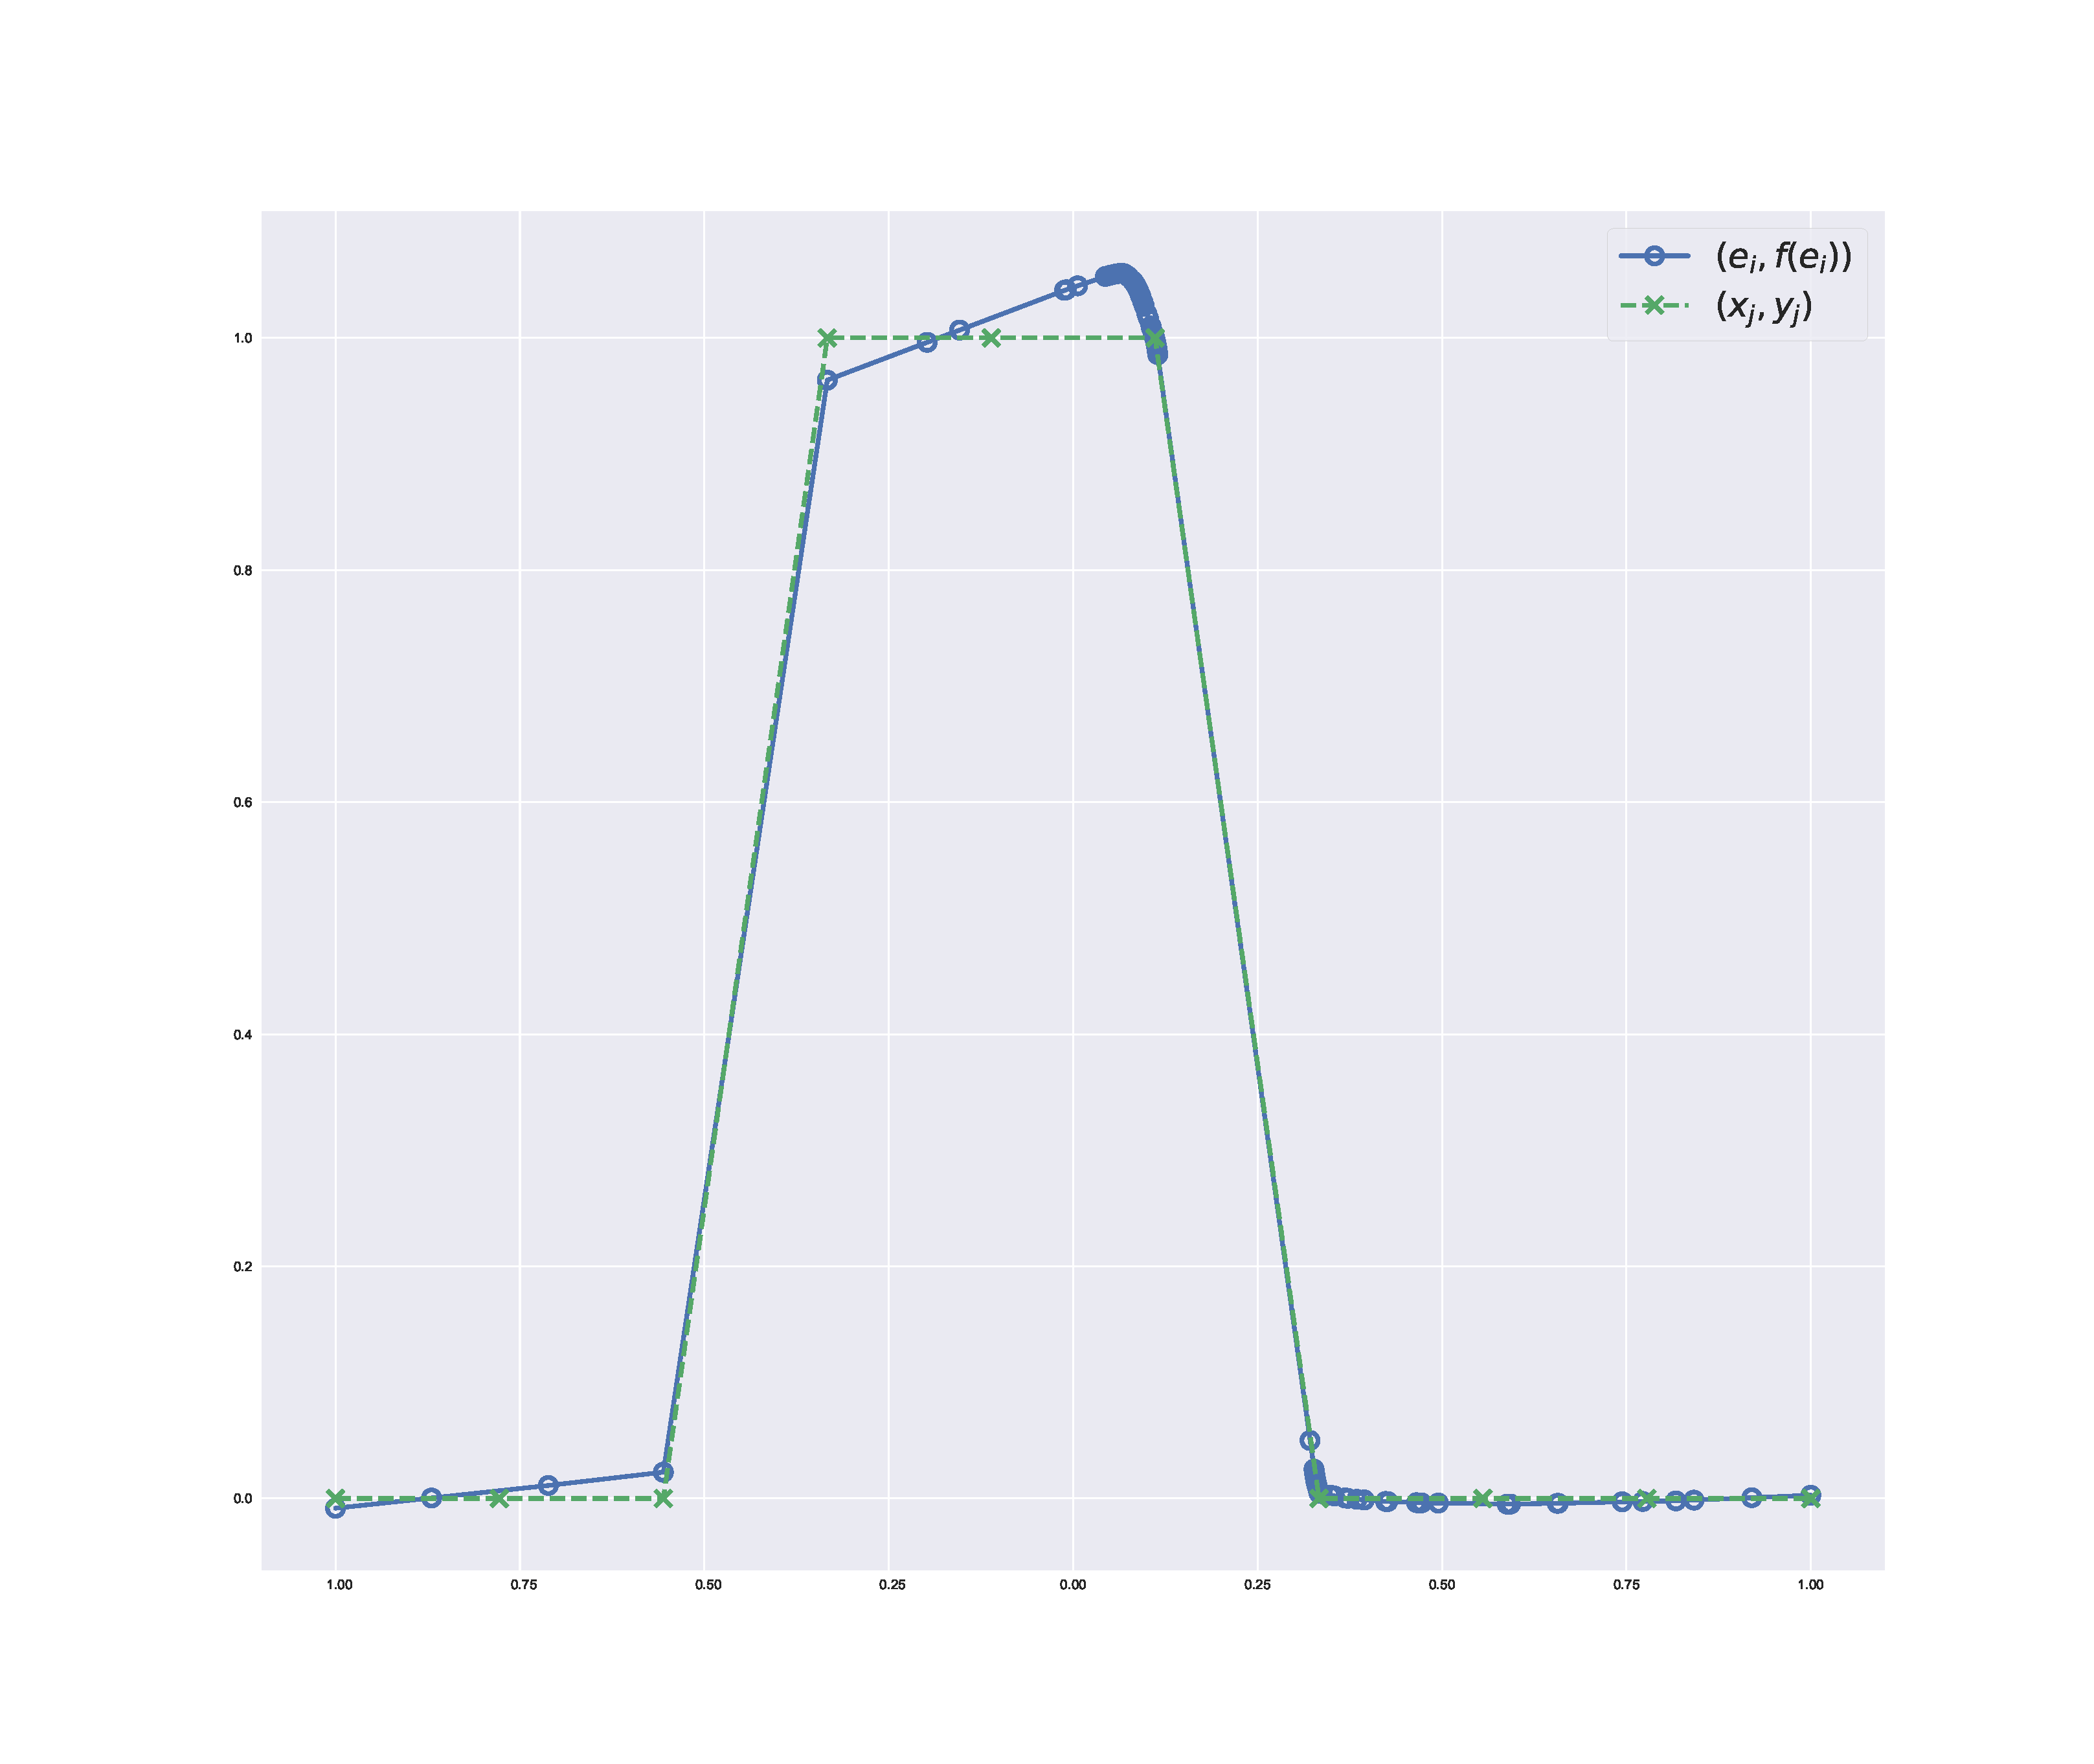
\includegraphics[width=\linewidth]{figures/neuron_trajectories_recon.pdf}
    \endminipage\hfill
    \minipage{0.33\textwidth}
    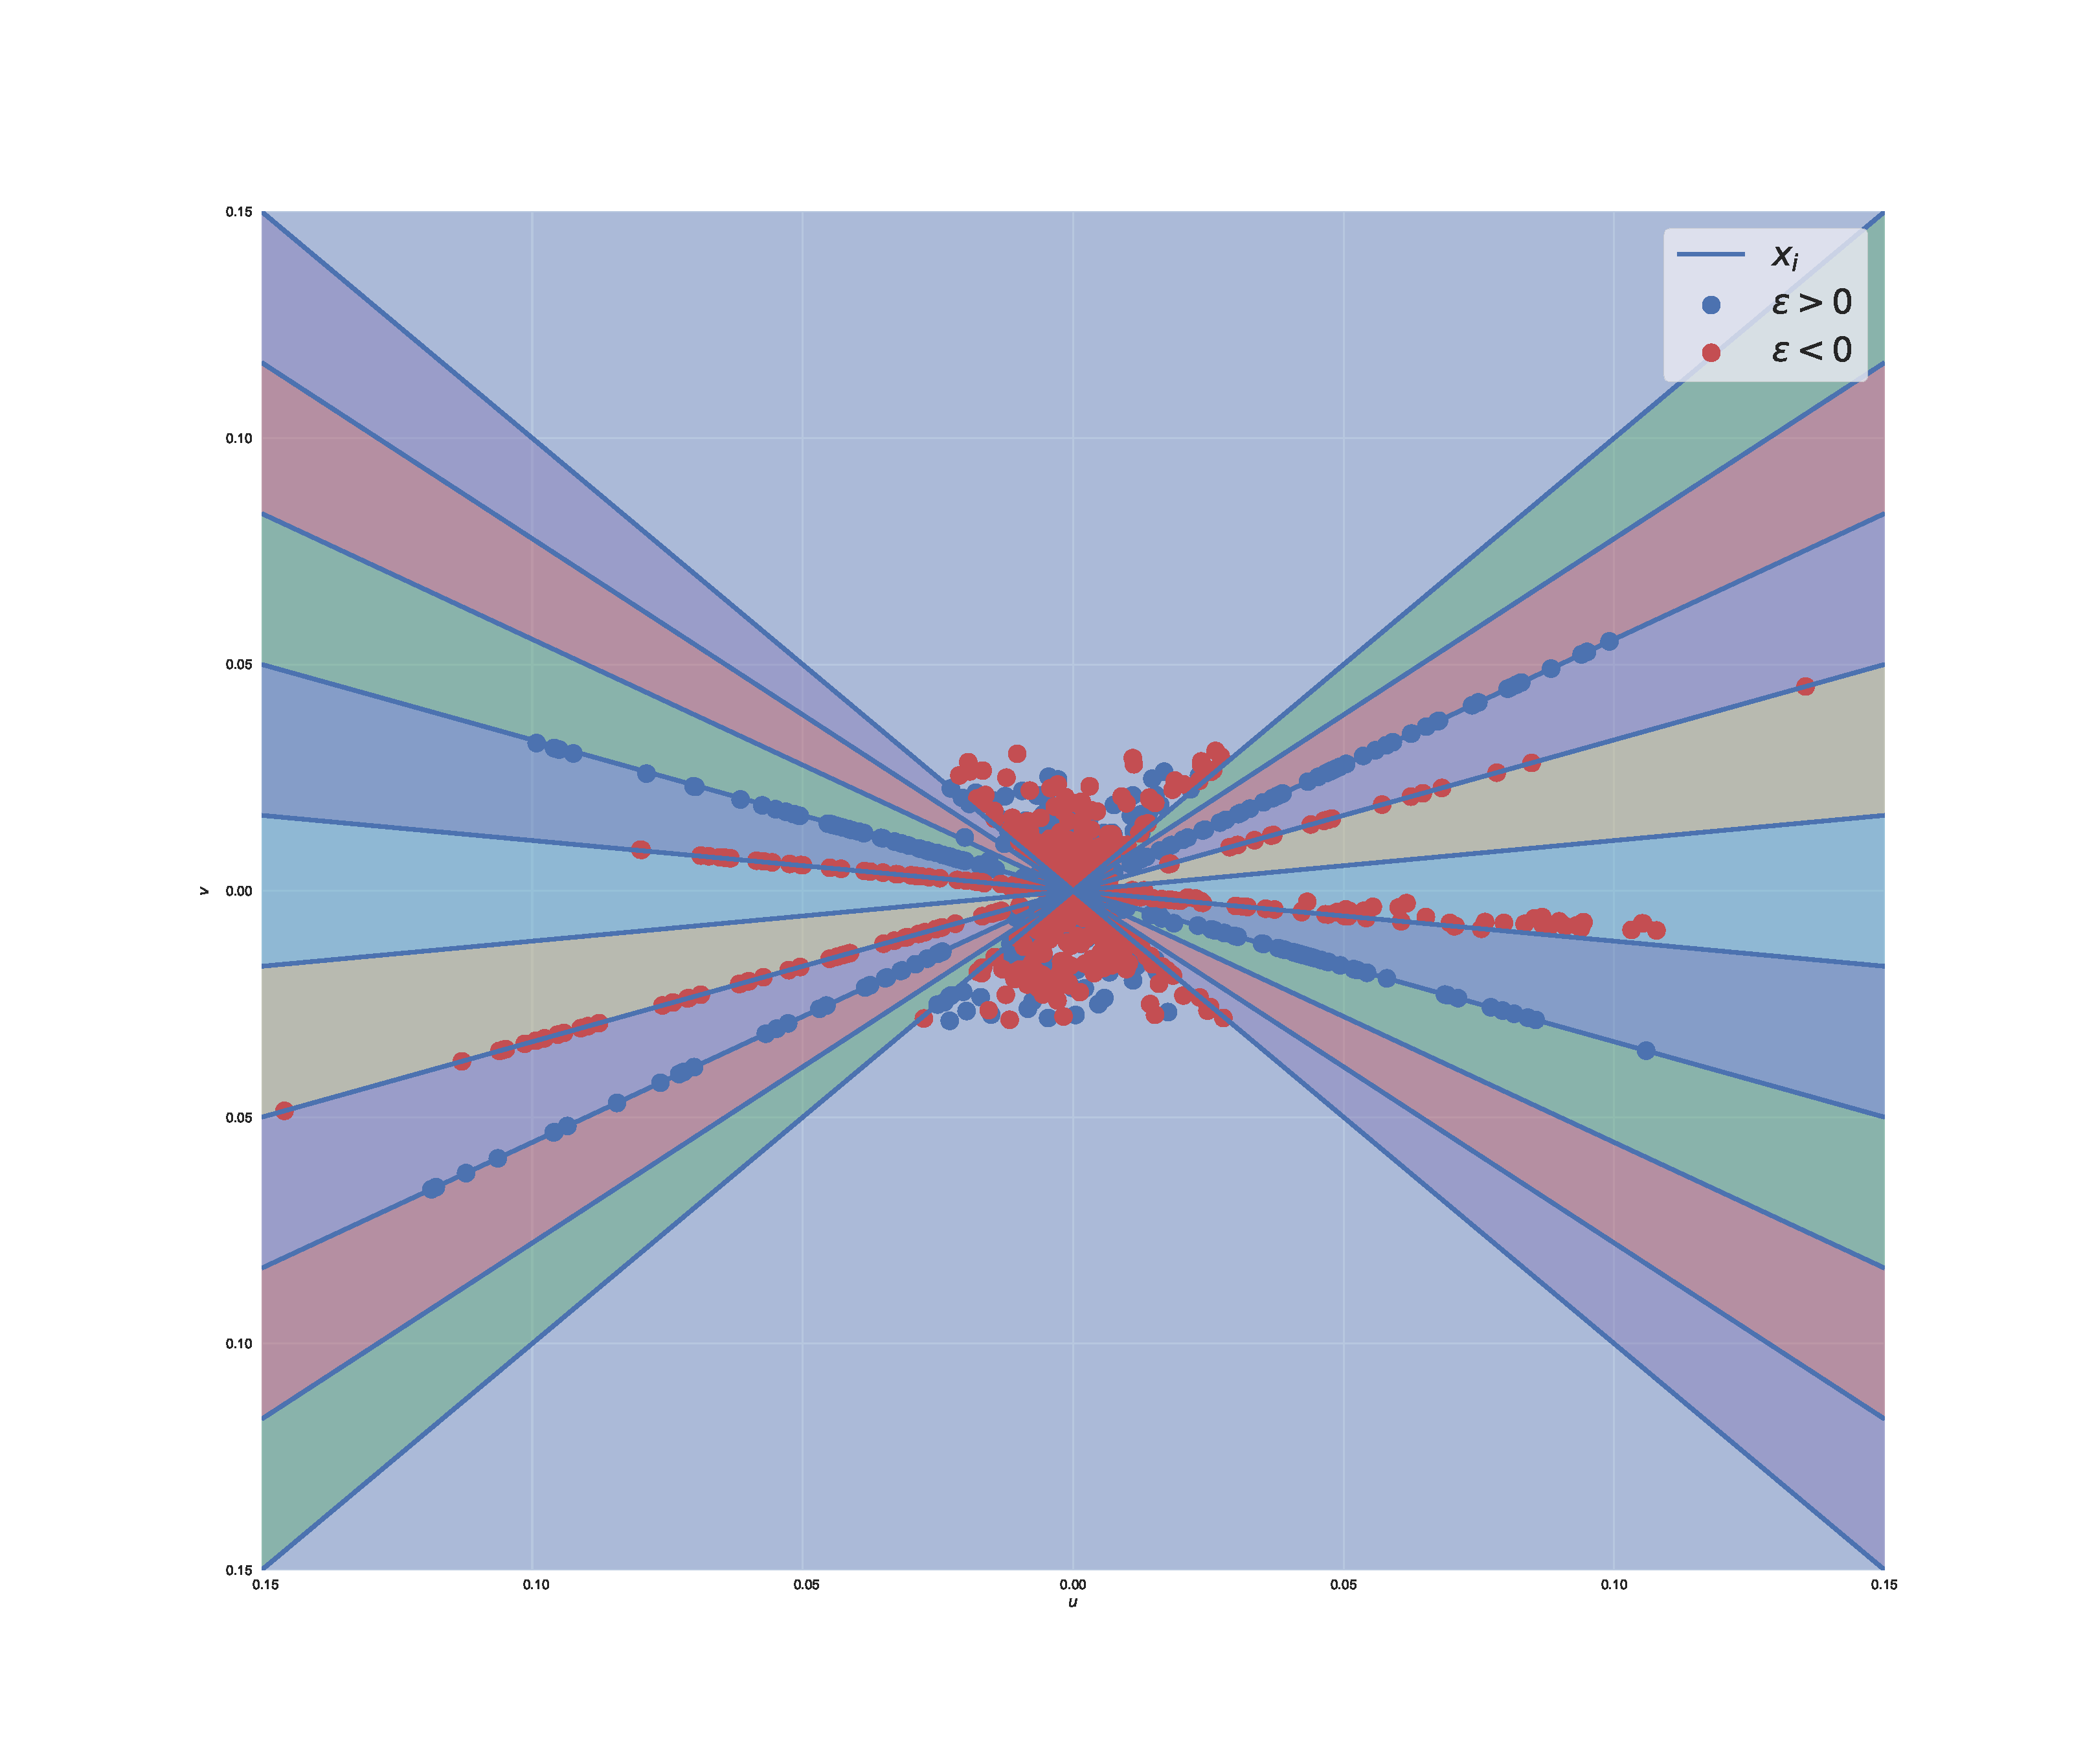
\includegraphics[width=\linewidth]{figures/neuron_trajectories_phase.pdf}
    \endminipage\hfill
    \minipage{0.33\textwidth}
    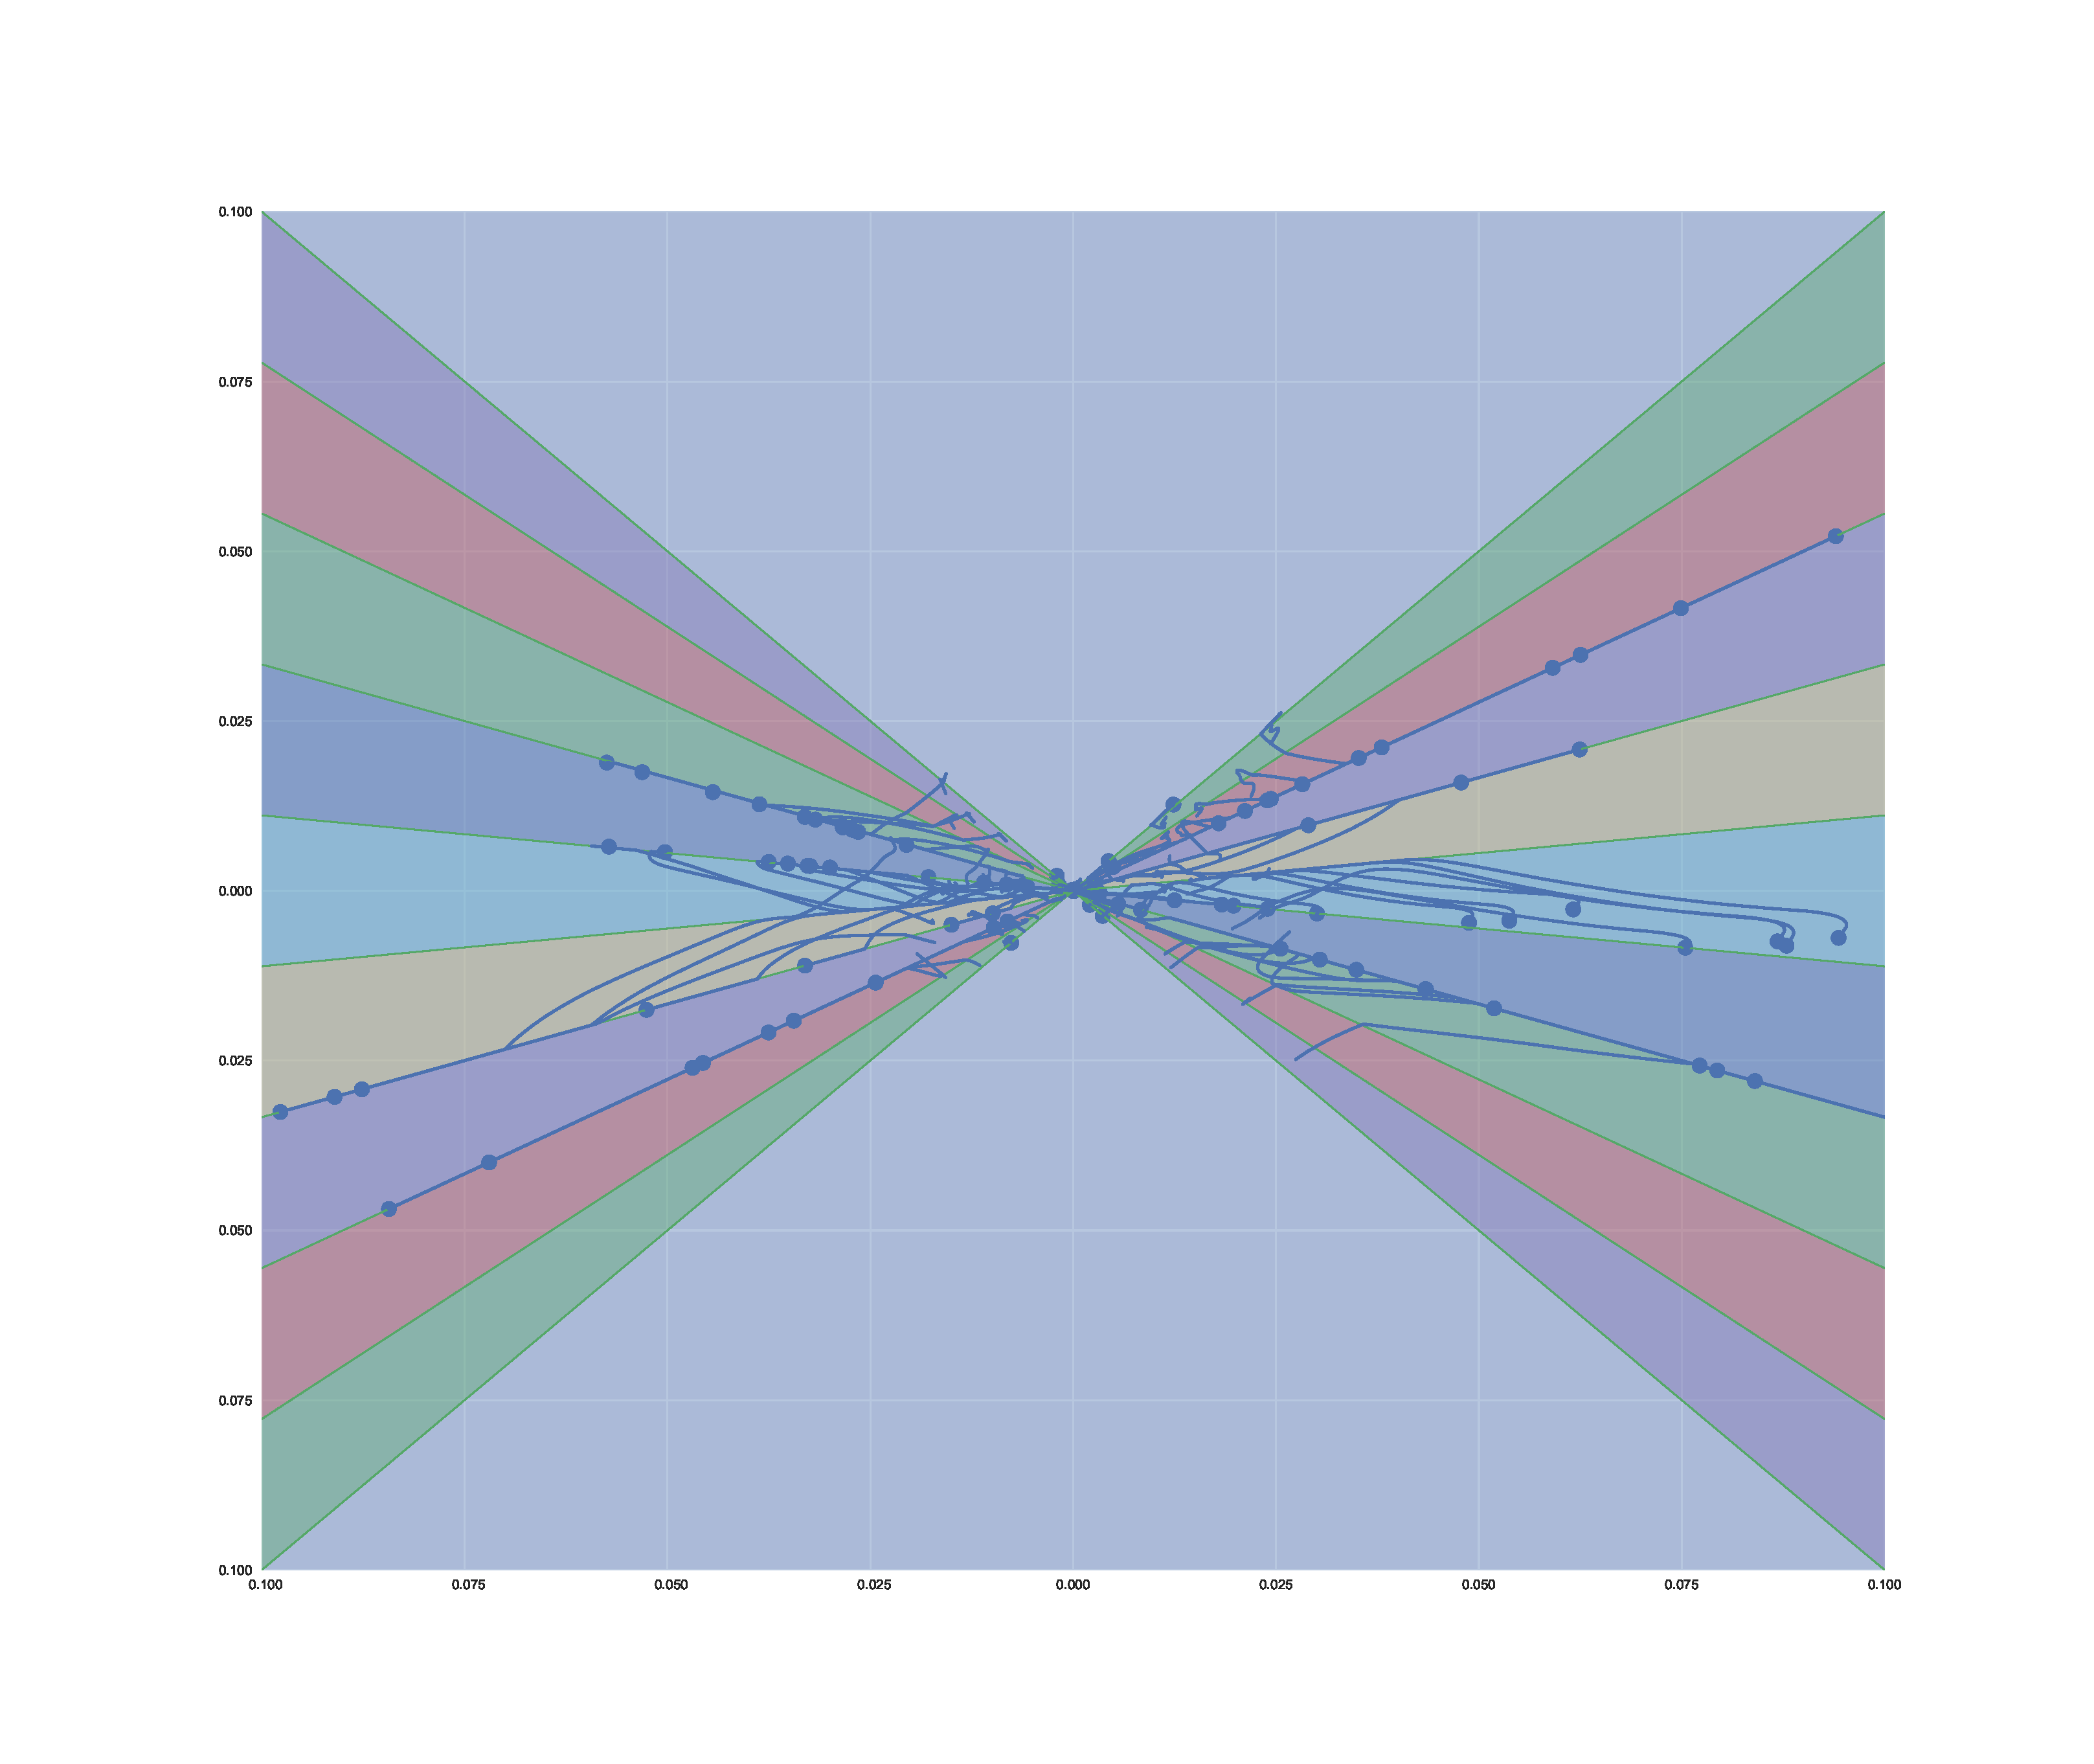
\includegraphics[width=\linewidth]{figures/neuron_trajectories.pdf}
    \endminipage
    \caption{Evolution of neurons in the tangential regime while fitting a square wave with 1000 neurons. The left image shows the trained network on and sample points. The middle image shows the distribution of all neurons at the end of training. The right image shows trajectories for a random sample of 100 neurons. Observe how in this regime, neurons concentrate on certain samples. The trajectories in this case get stuck at the sample boundary.}
    \label{fig:tangential_trajectories}
\end{figure}


\begin{figure}
    \centering
    \minipage{0.33\textwidth}
    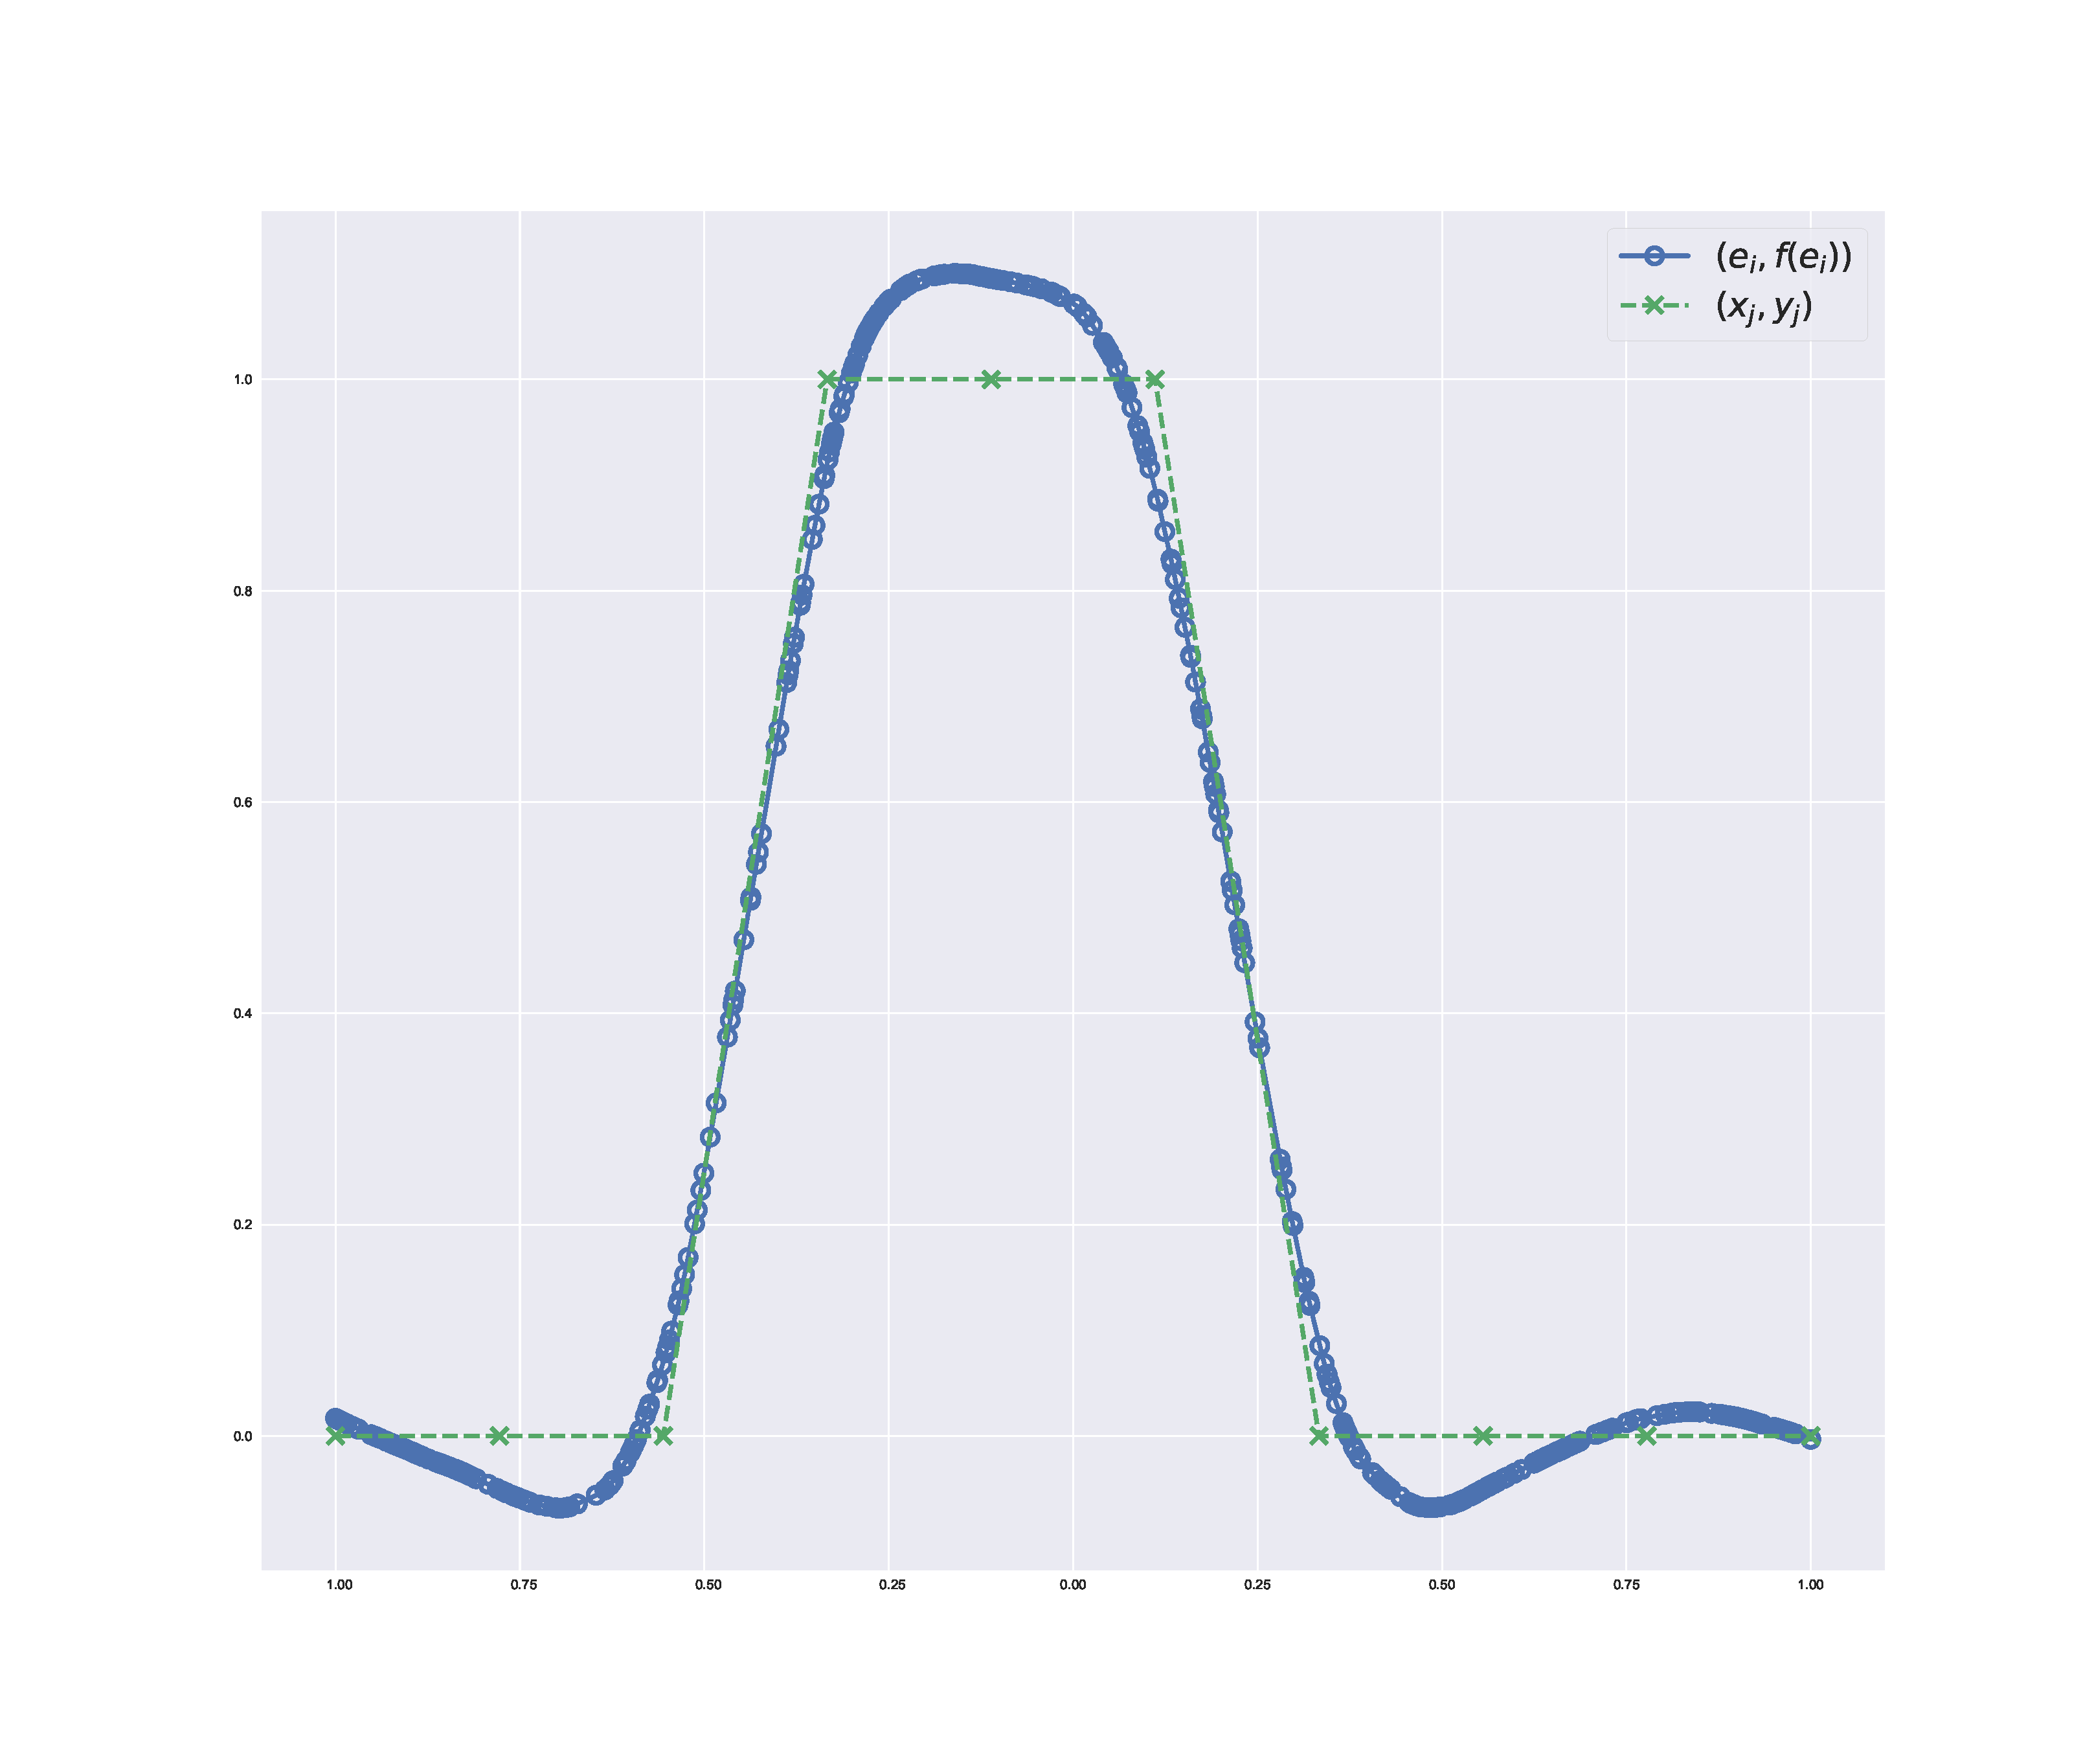
\includegraphics[width=\linewidth]{figures/radial_trajectories_recon.pdf}
    \endminipage\hfill
    \minipage{0.33\textwidth}
    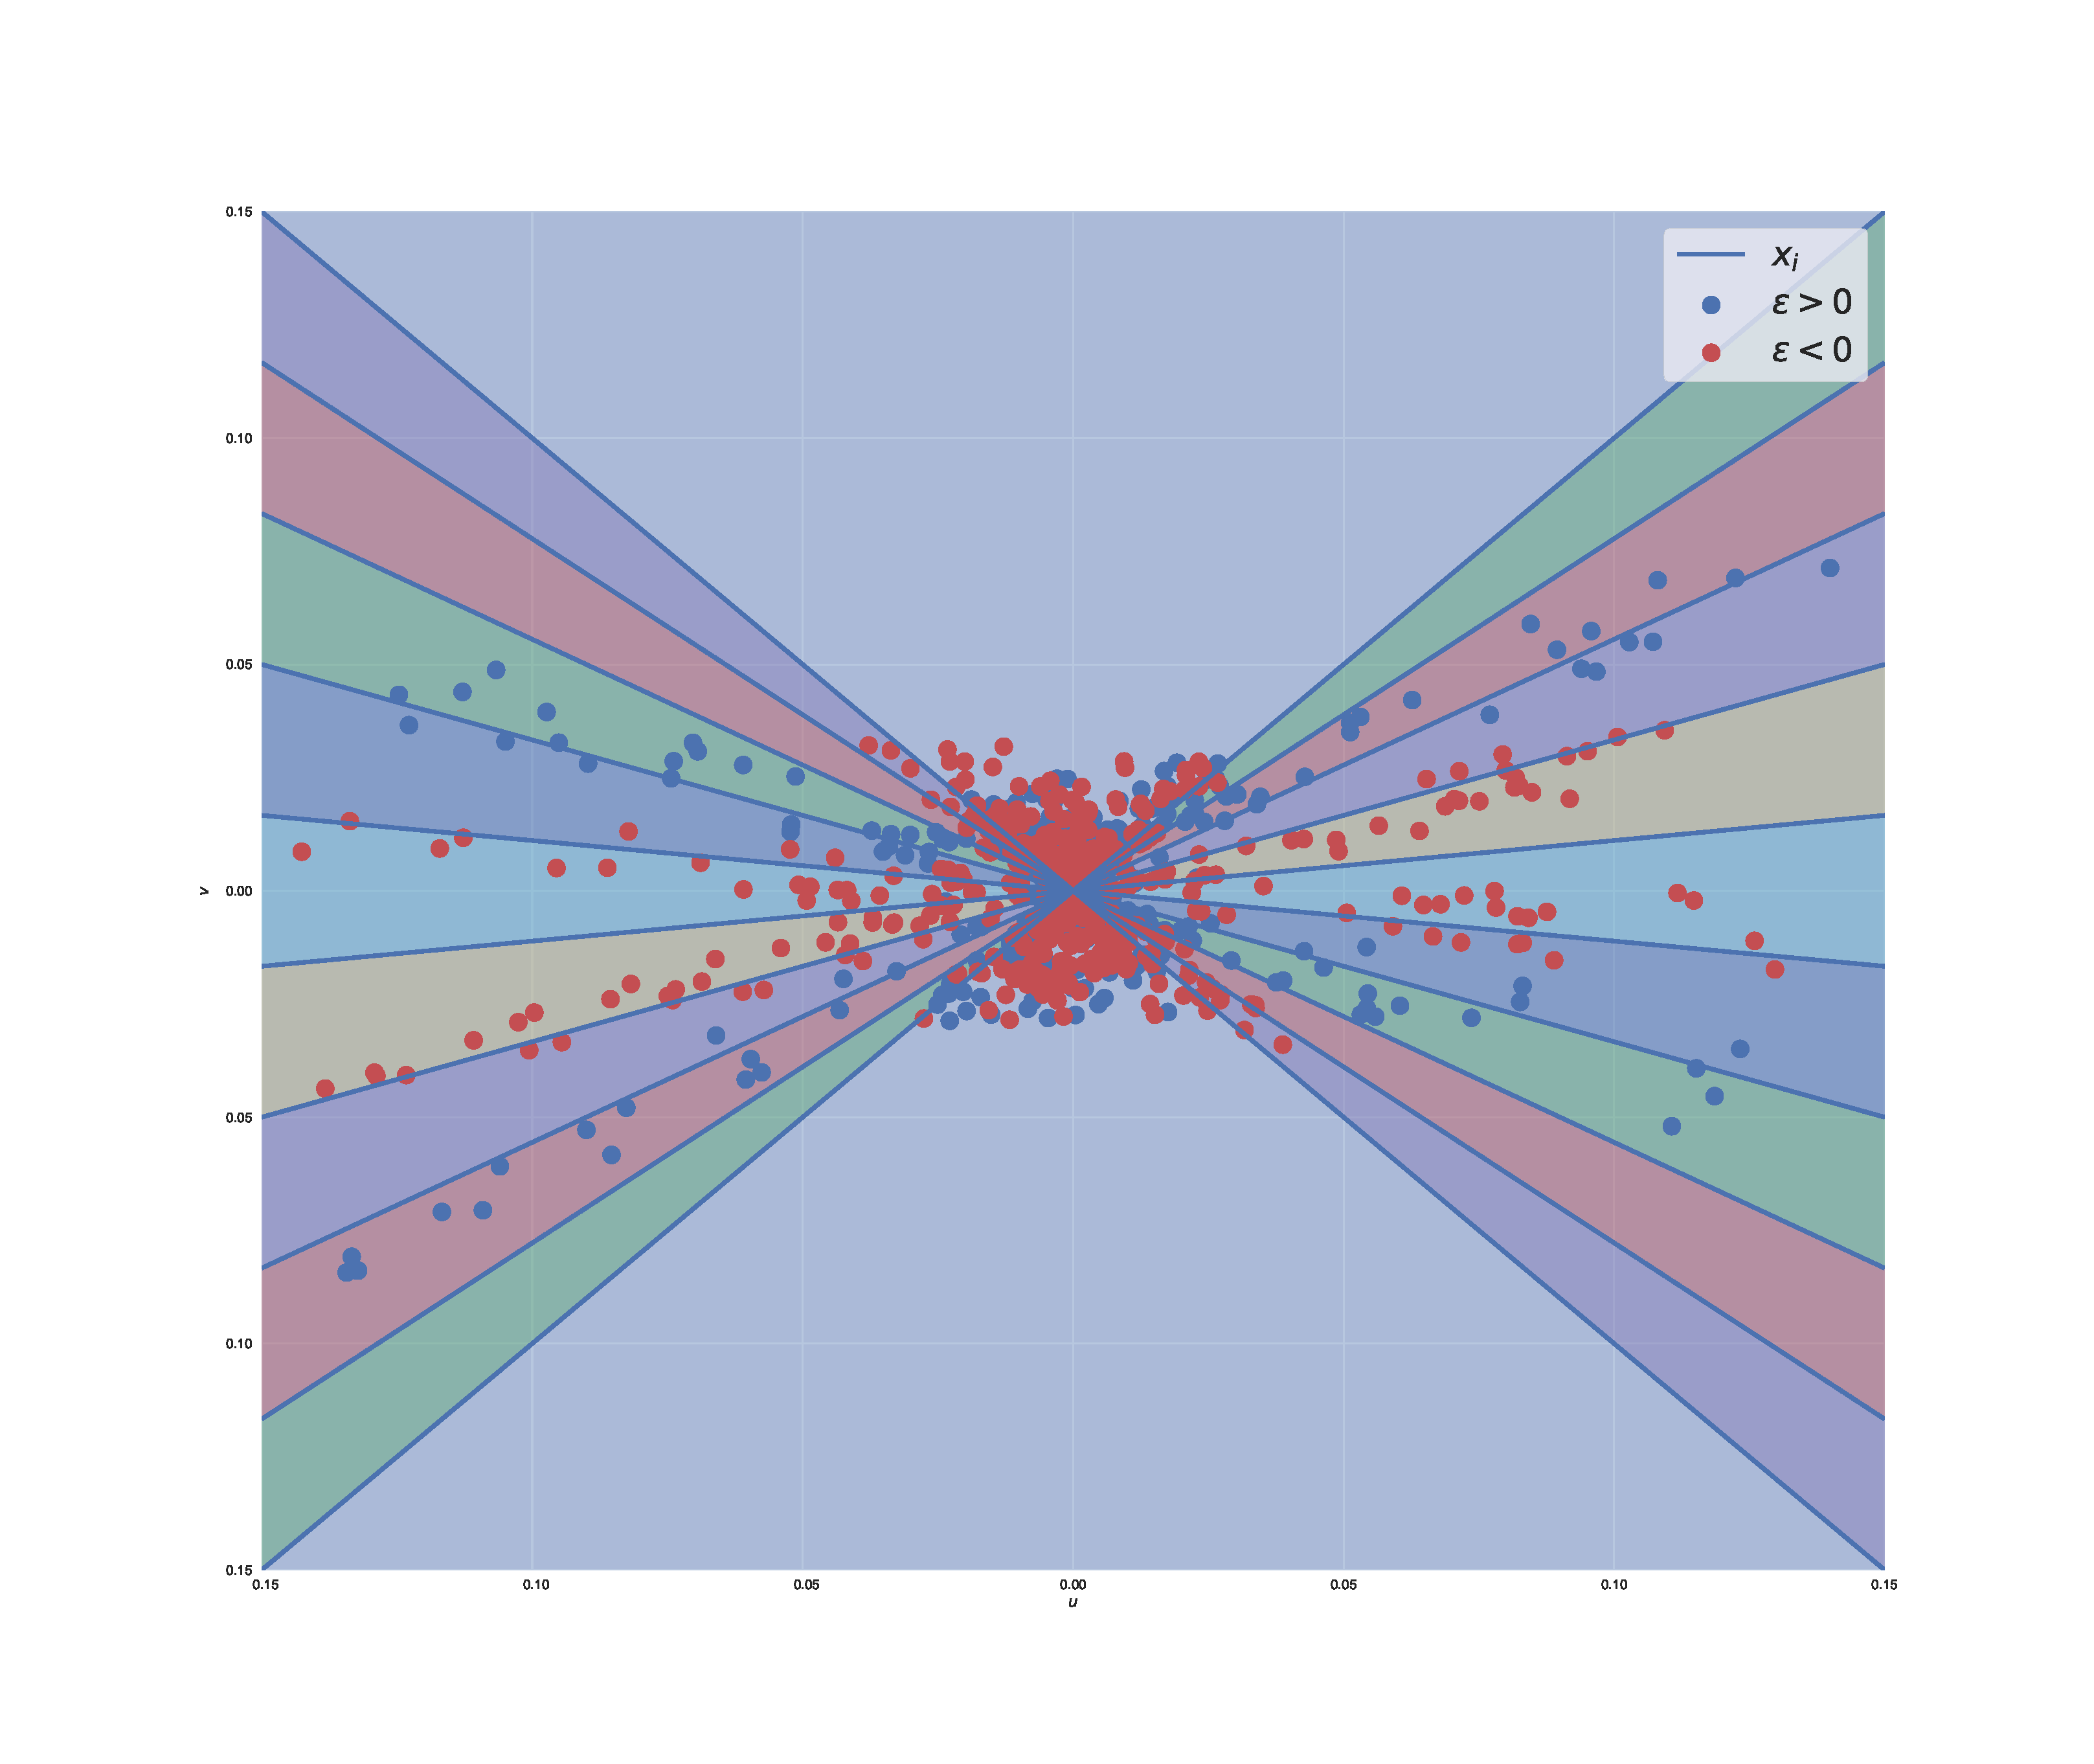
\includegraphics[width=\linewidth]{figures/radial_trajectories_phase.pdf}
    \endminipage\hfill
    \minipage{0.33\textwidth}
    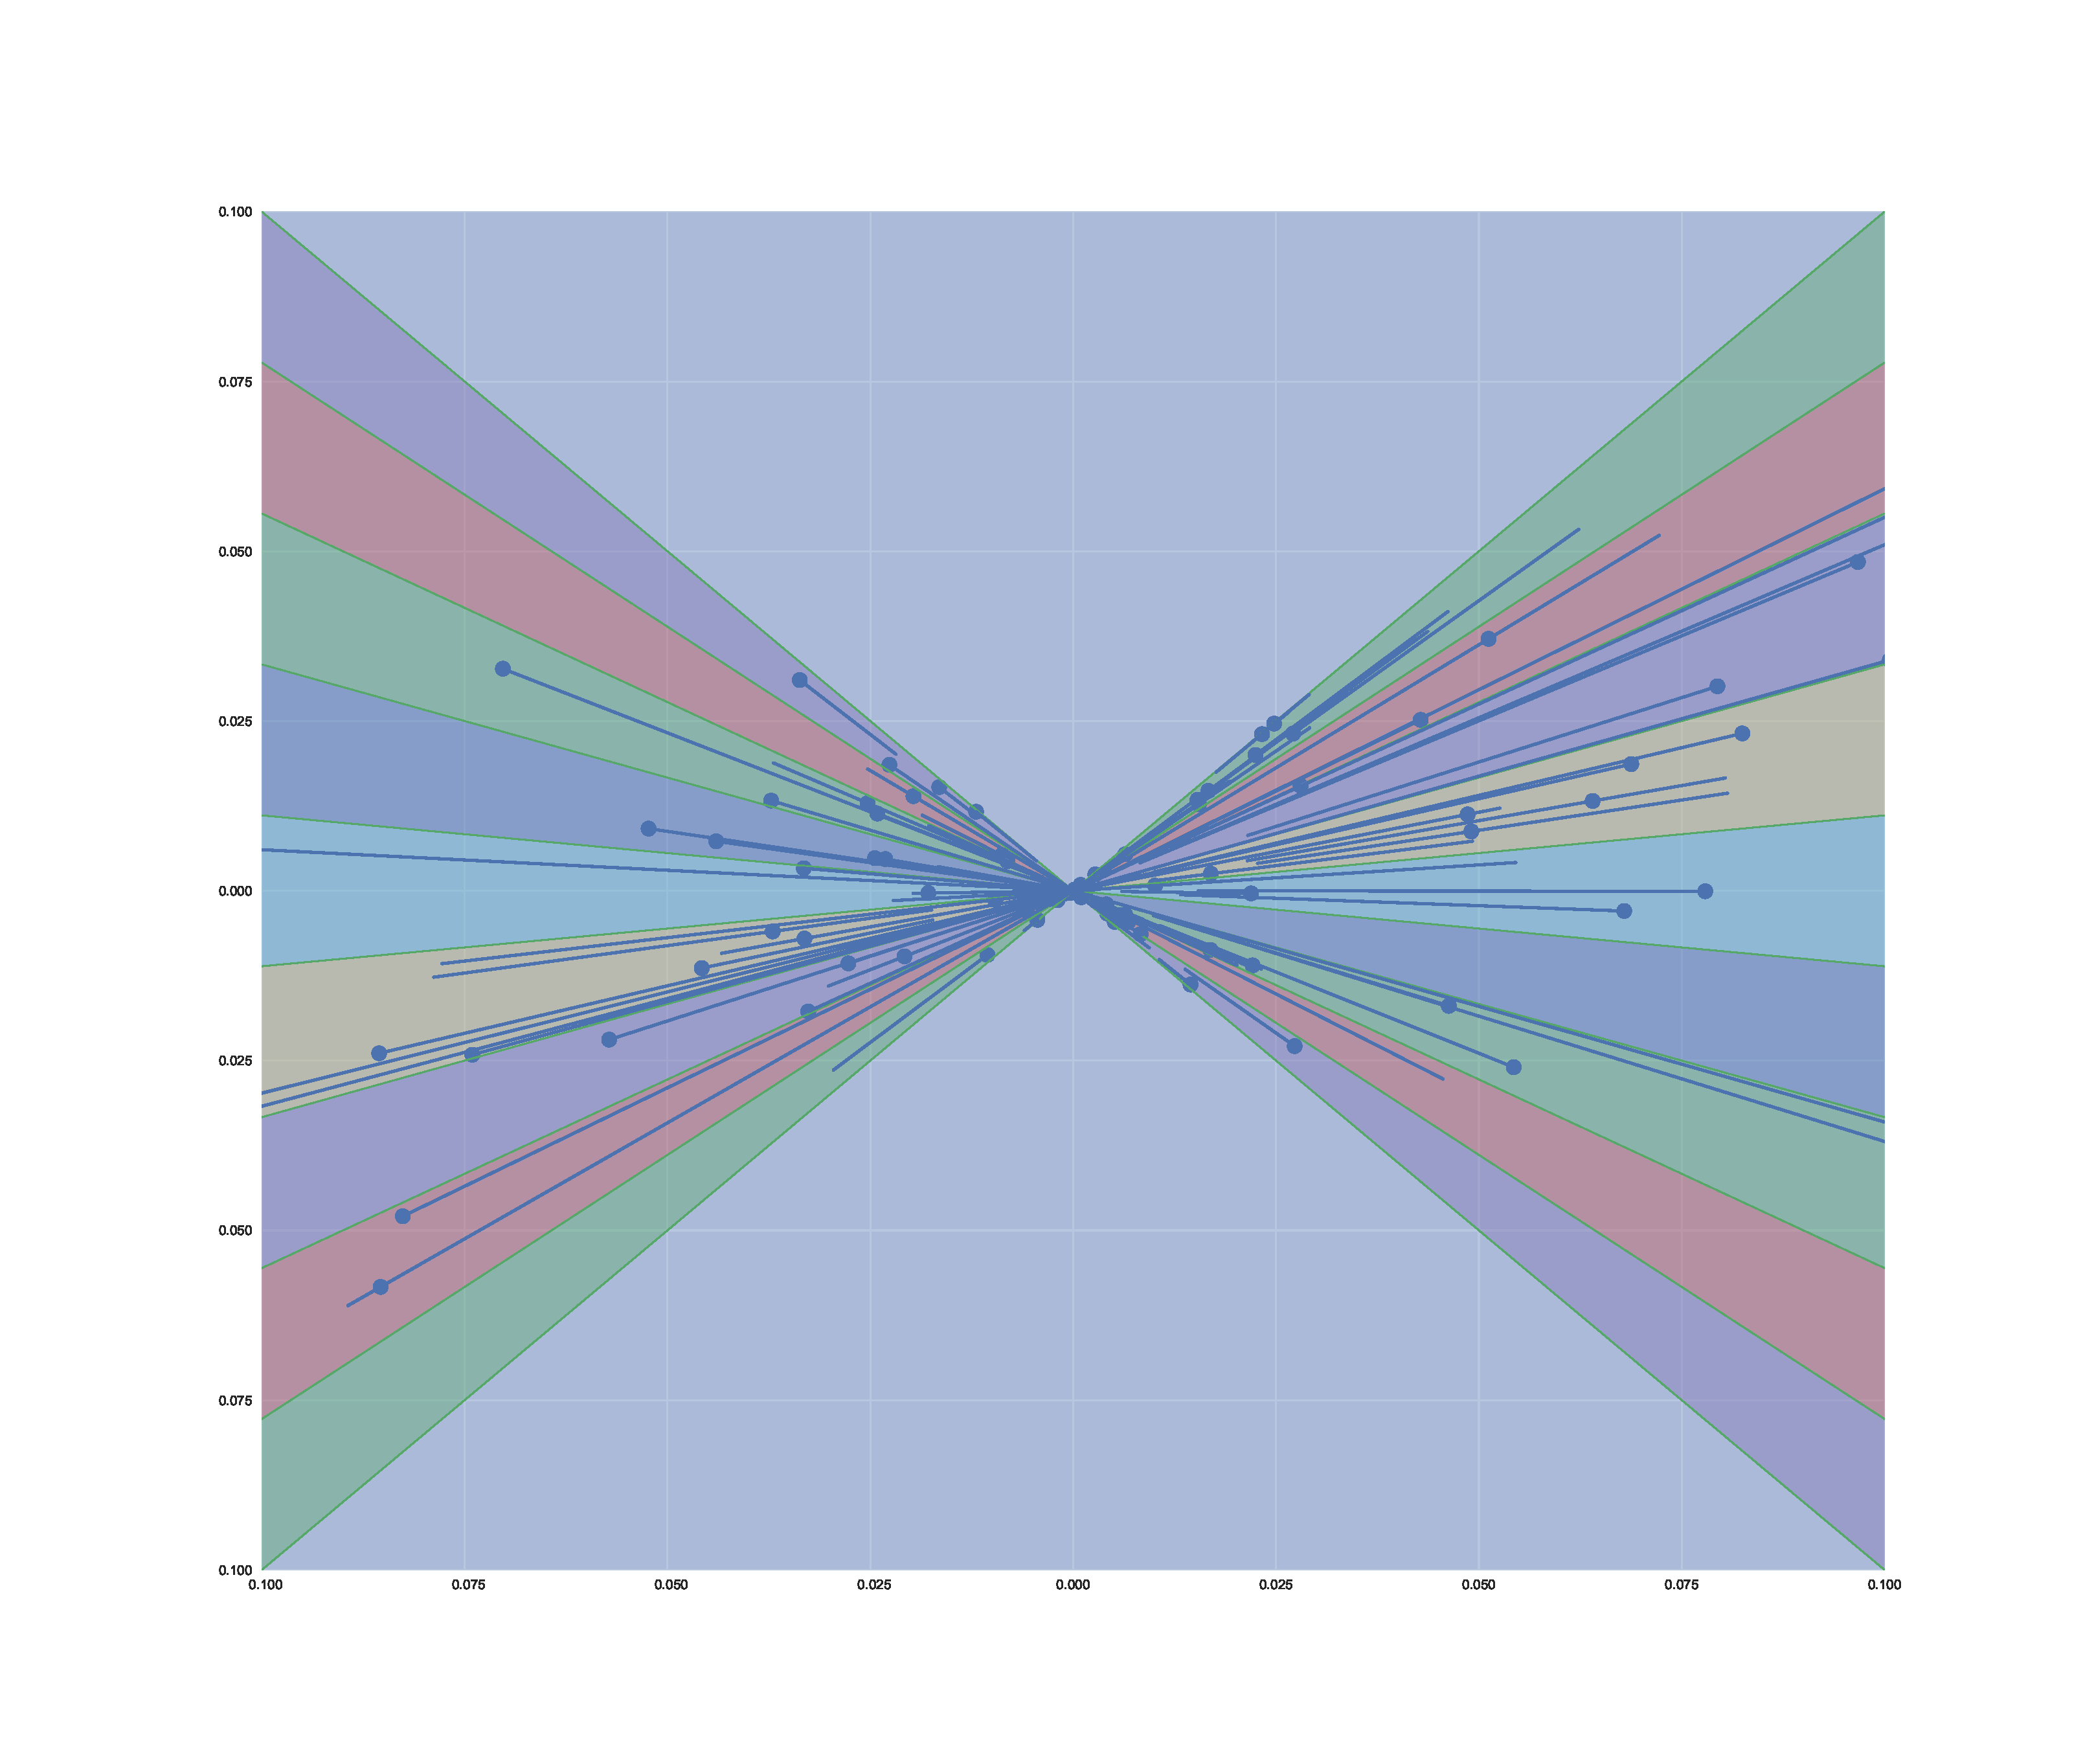
\includegraphics[width=\linewidth]{figures/radial_trajectories.pdf}
    \endminipage
    \caption{Evolution of neurons in the radial regime while fitting a square wave with 1000 neurons. The left image shows the trained network on and sample points. The middle image shows the distribution of all neurons at the end of training. The right image shows trajectories for a random sample of 100 neurons.}
    \label{fig:radial_trajectores}
\end{figure}


\begin{figure}\label{fig:different_funcs_same_init}
    \centering
    \minipage{0.33\textwidth}
    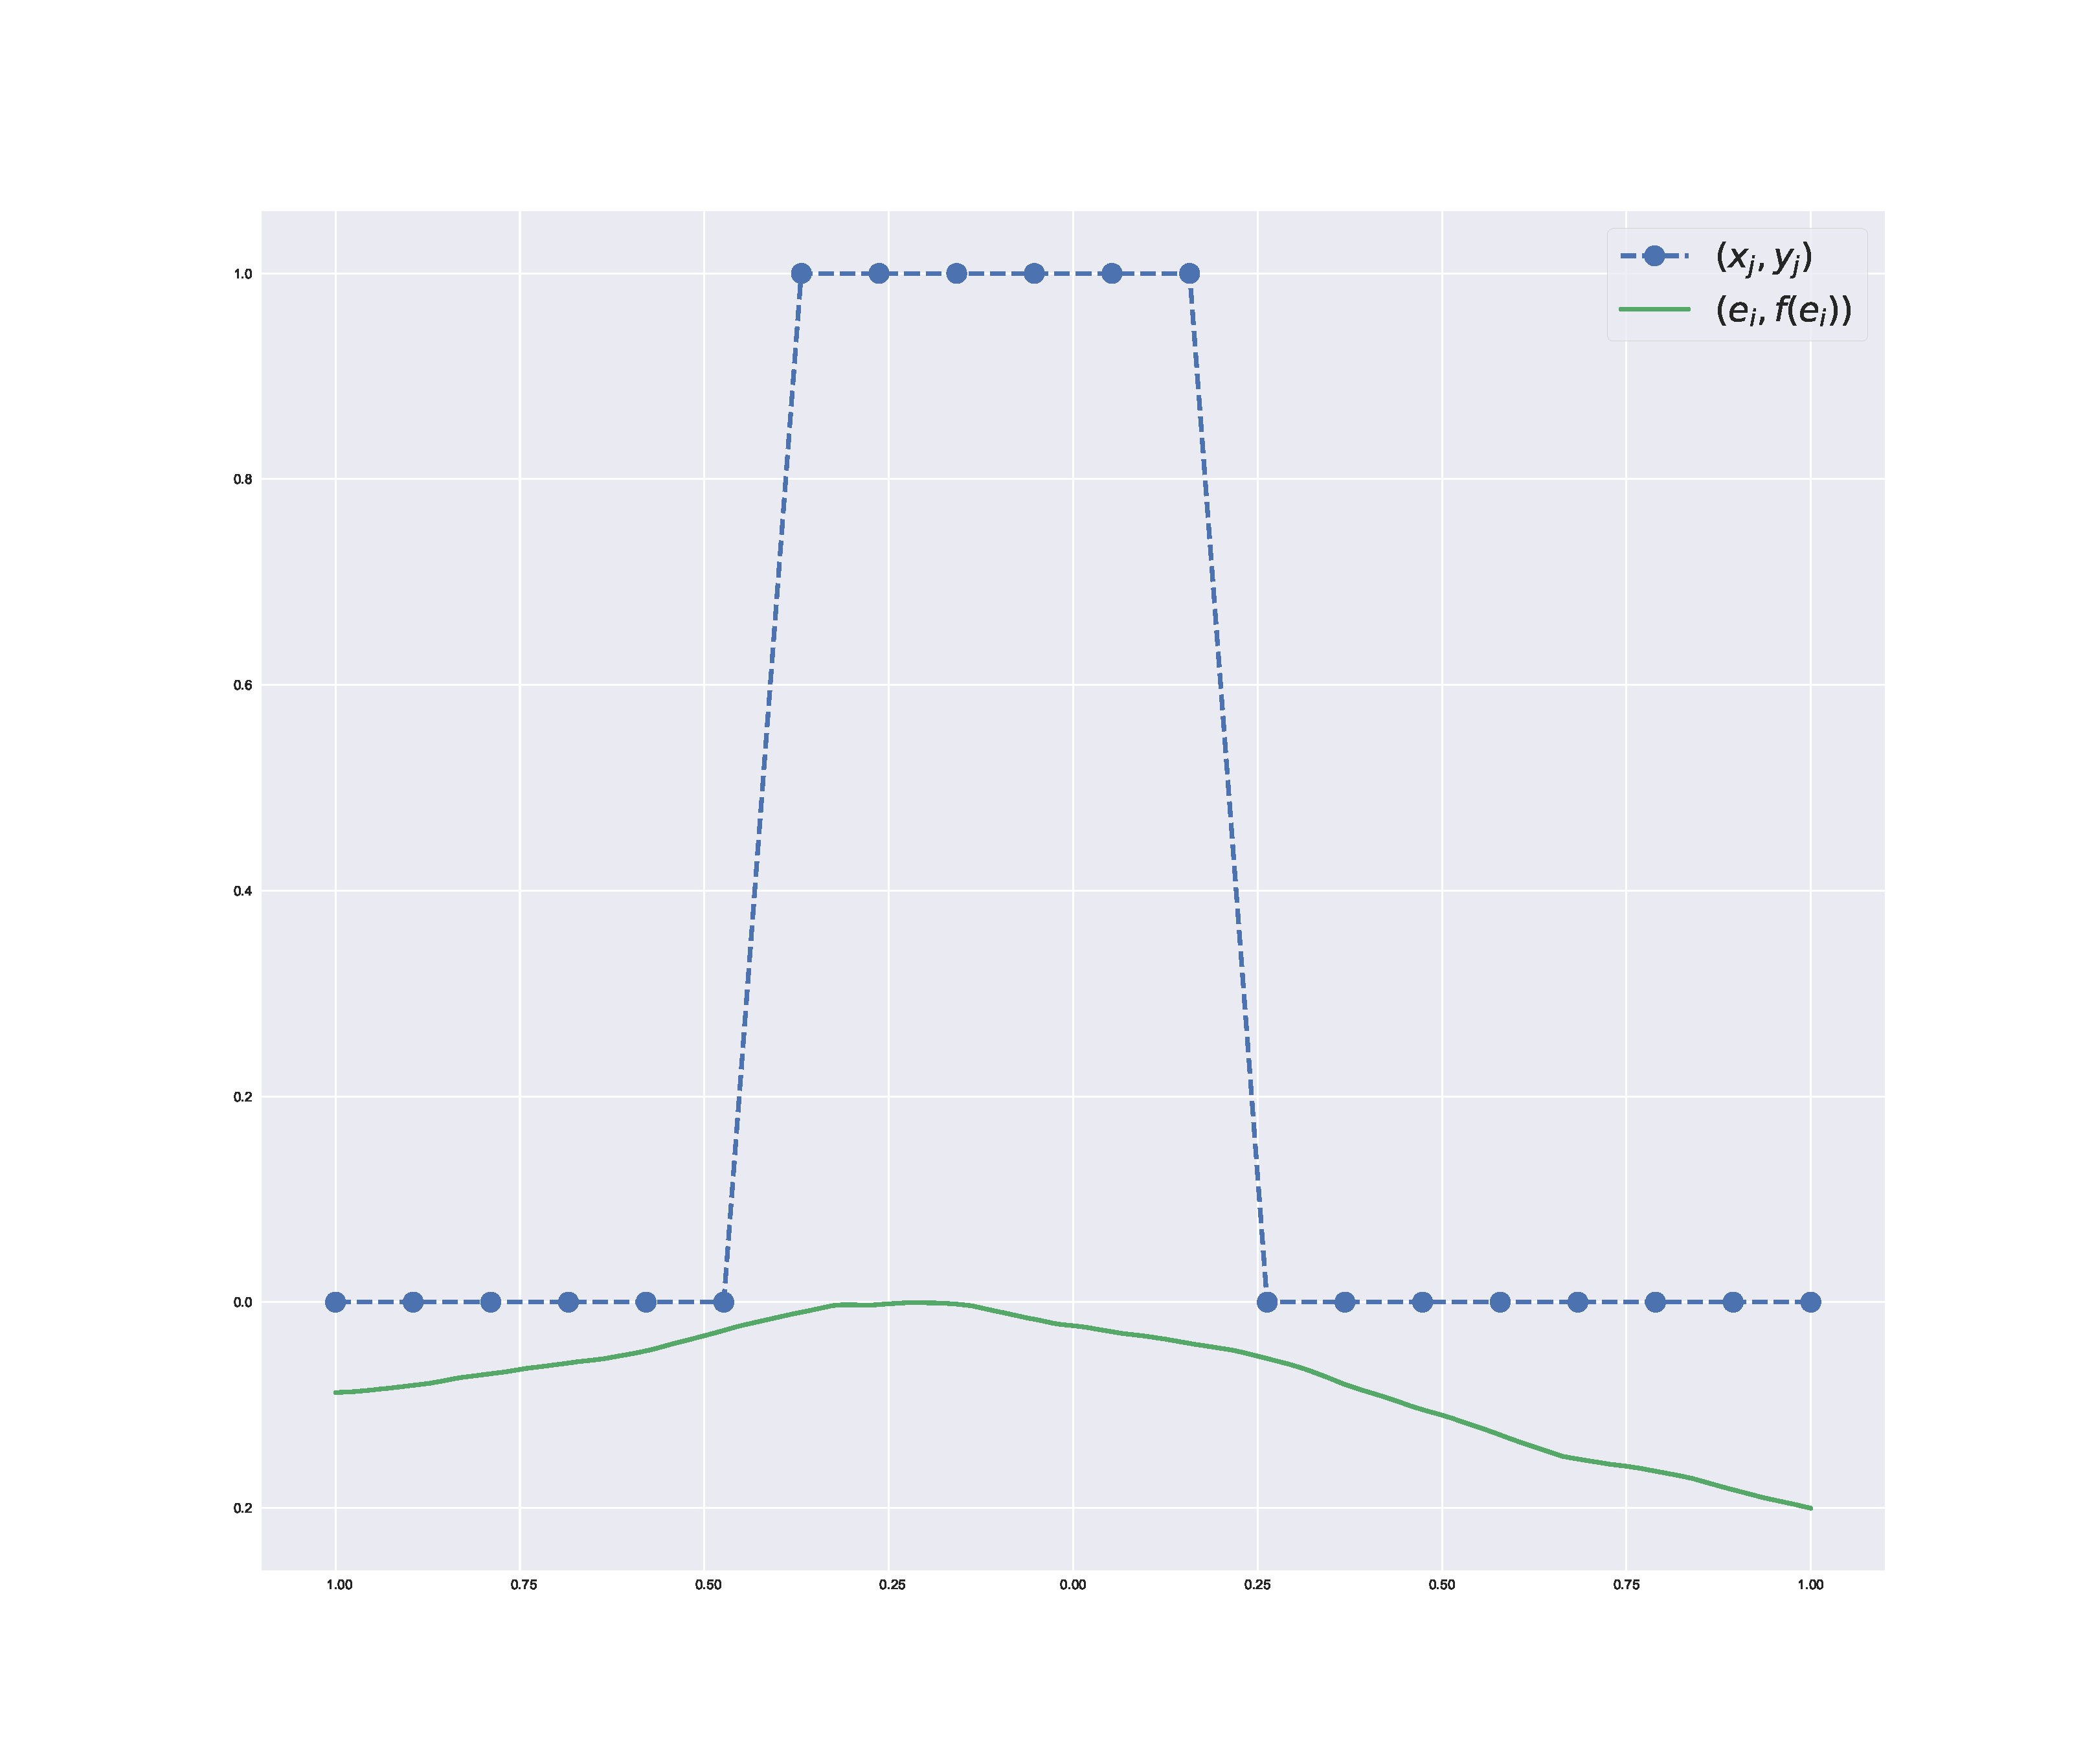
\includegraphics[width=\linewidth]{figures/same_init_different_func_square_init.pdf}
    \endminipage\hfill
    % \minipage{0.2\textwidth}
    % 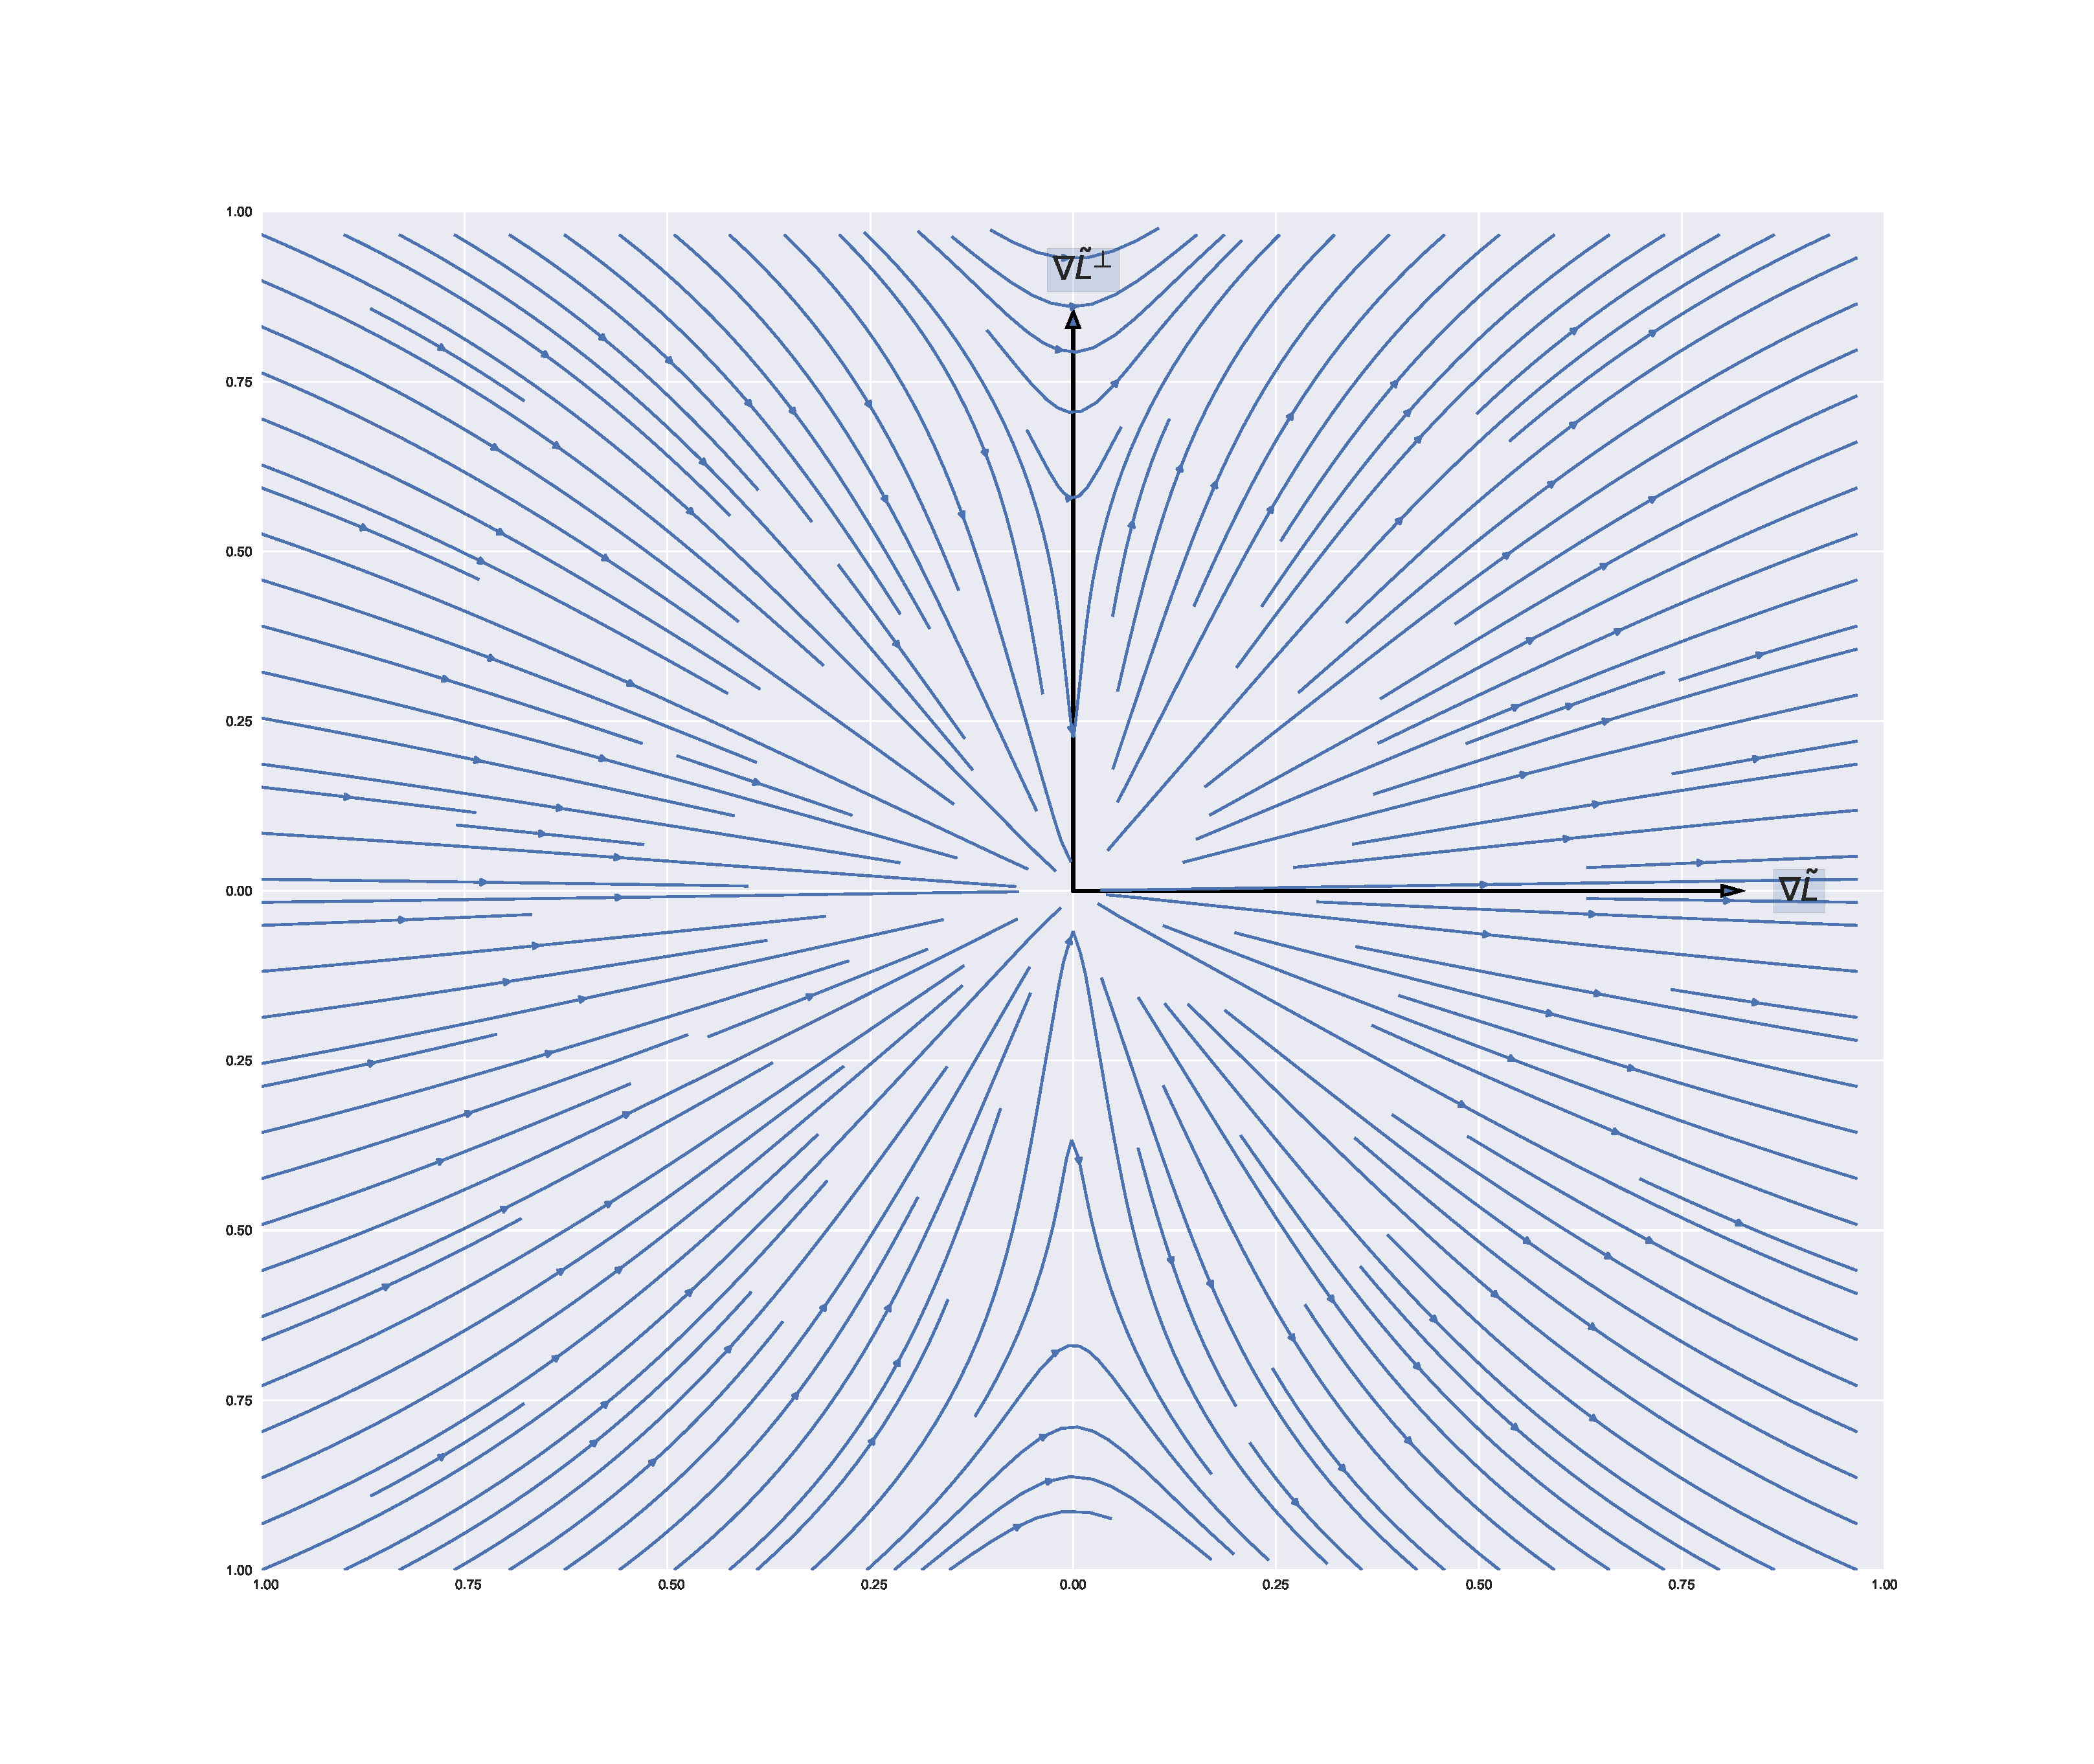
\includegraphics[width=\linewidth]{figures/dynamics_delta_-1.pdf}
    % \endminipage\hfill
    \minipage{0.33\textwidth}
    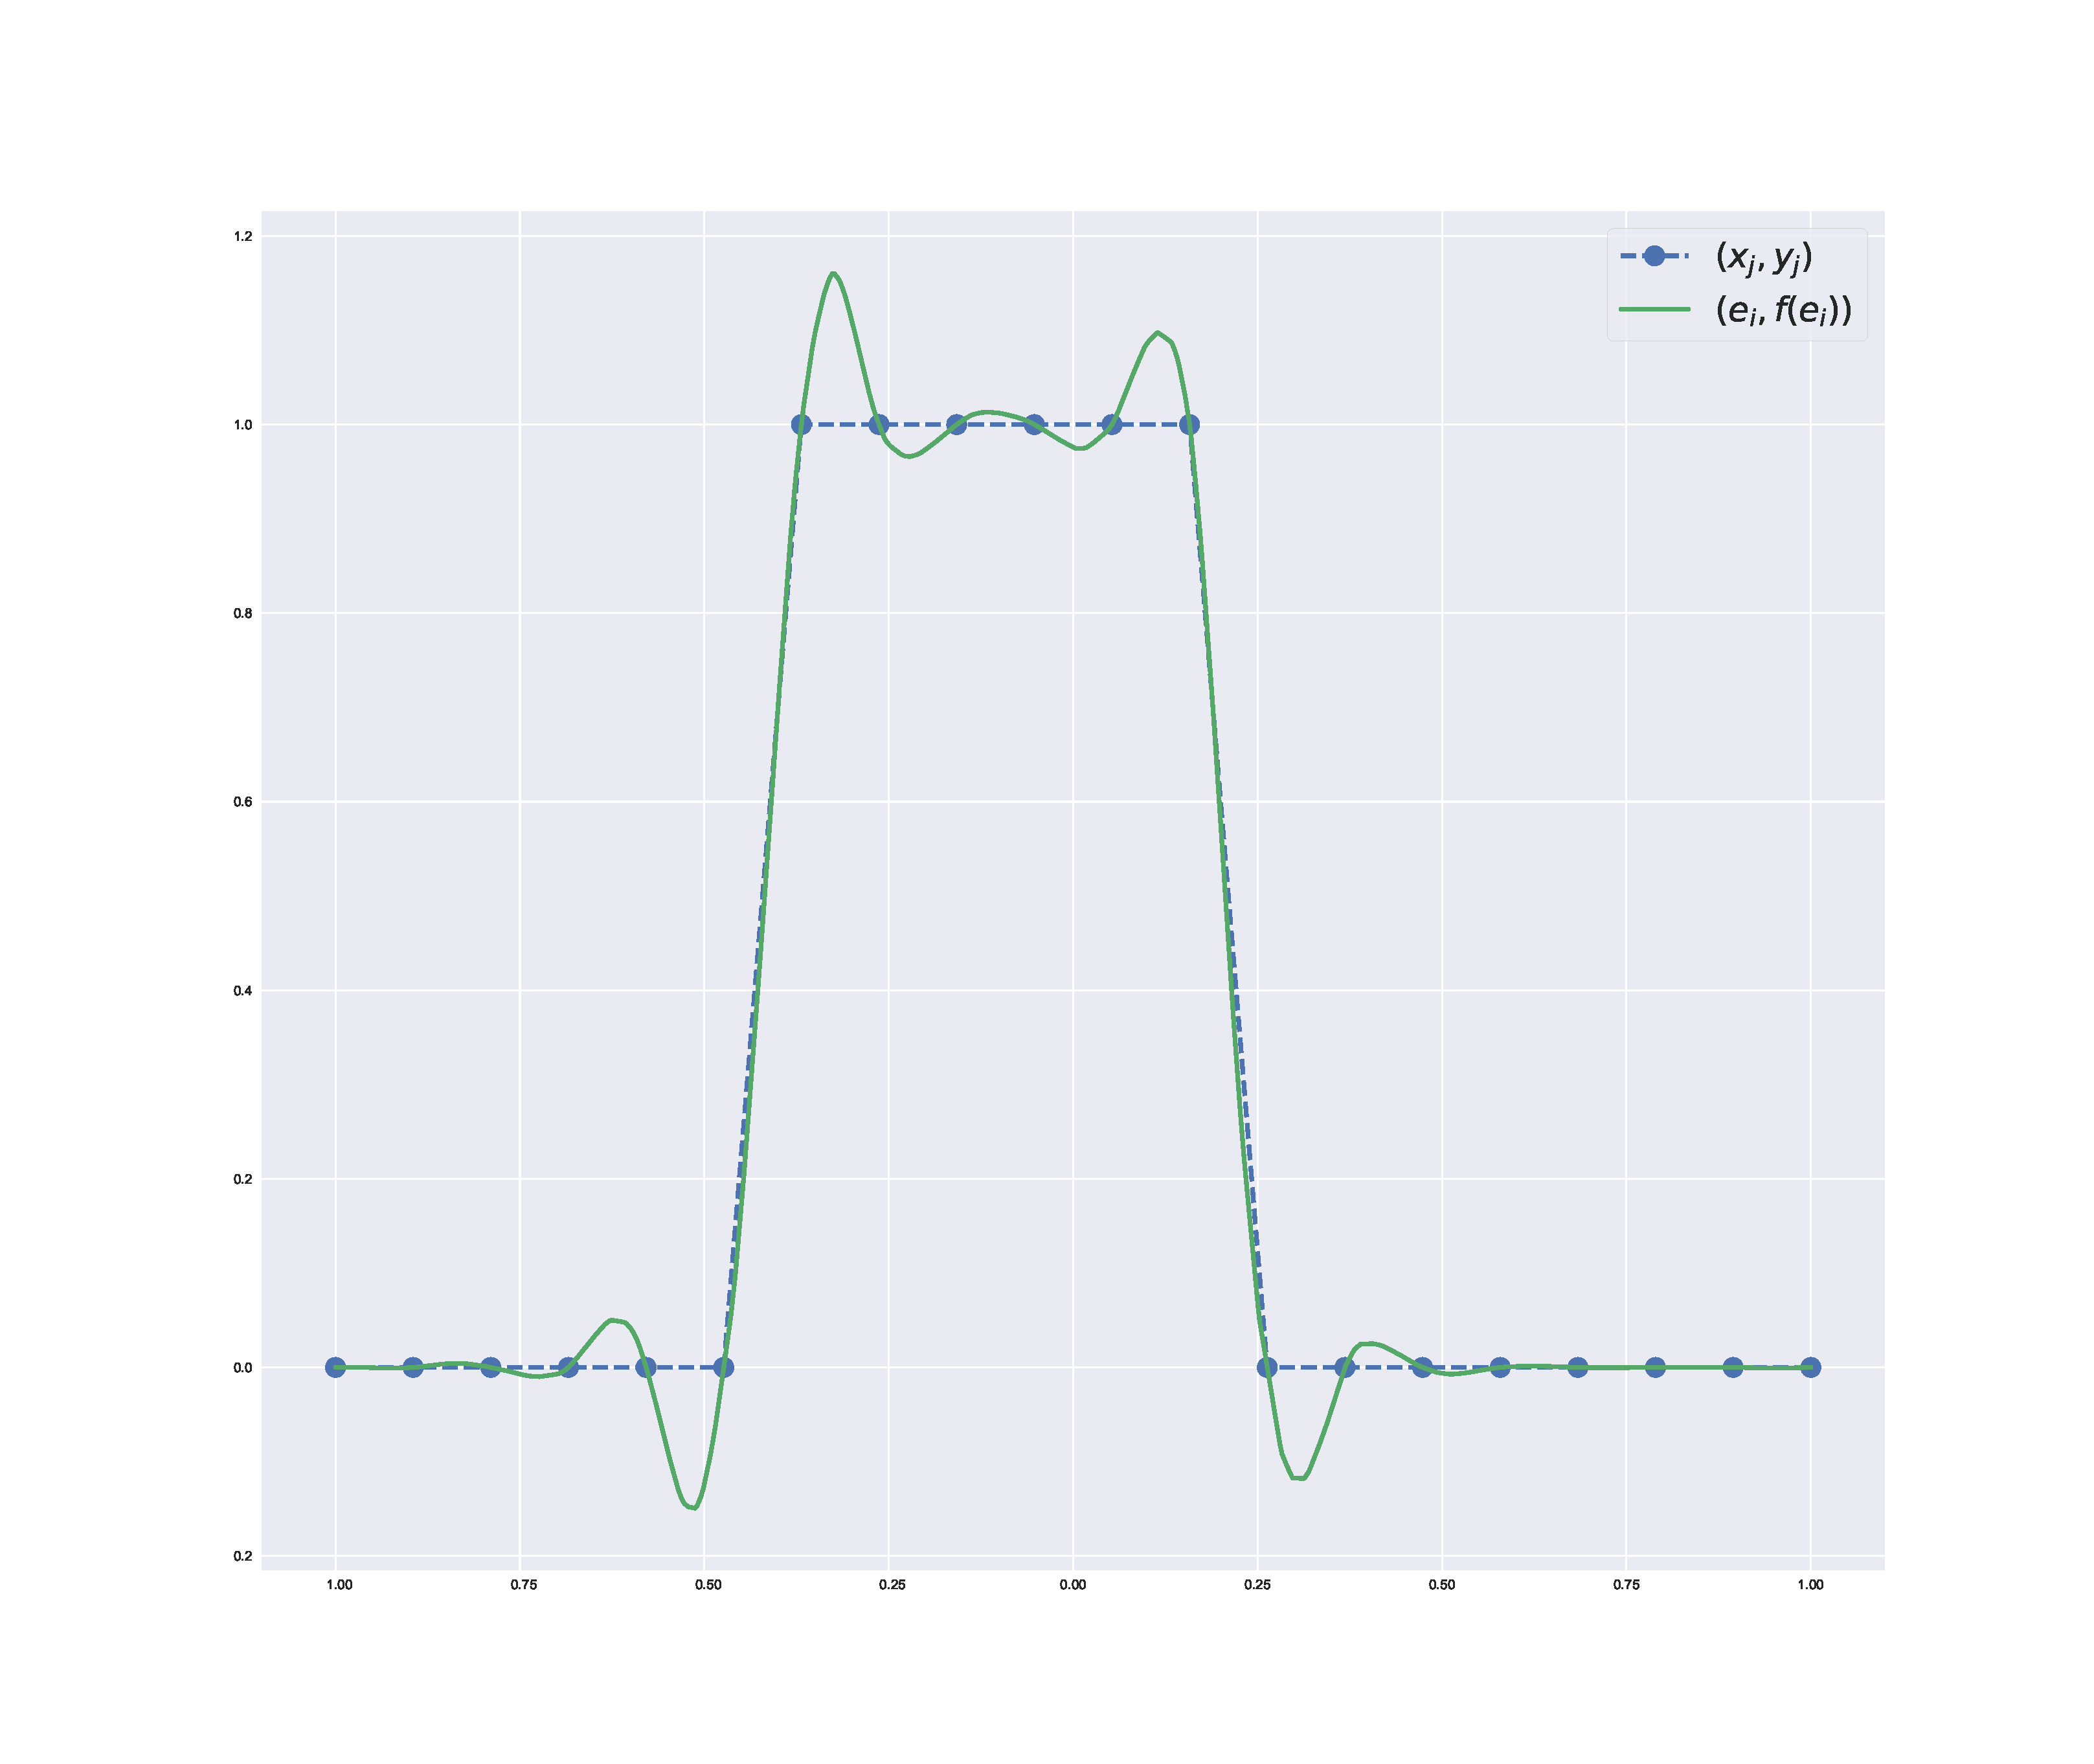
\includegraphics[width=\linewidth]{figures/same_init_different_func_square_1.pdf}
    \endminipage\hfill
    % \minipage{0.2\textwidth}
    % 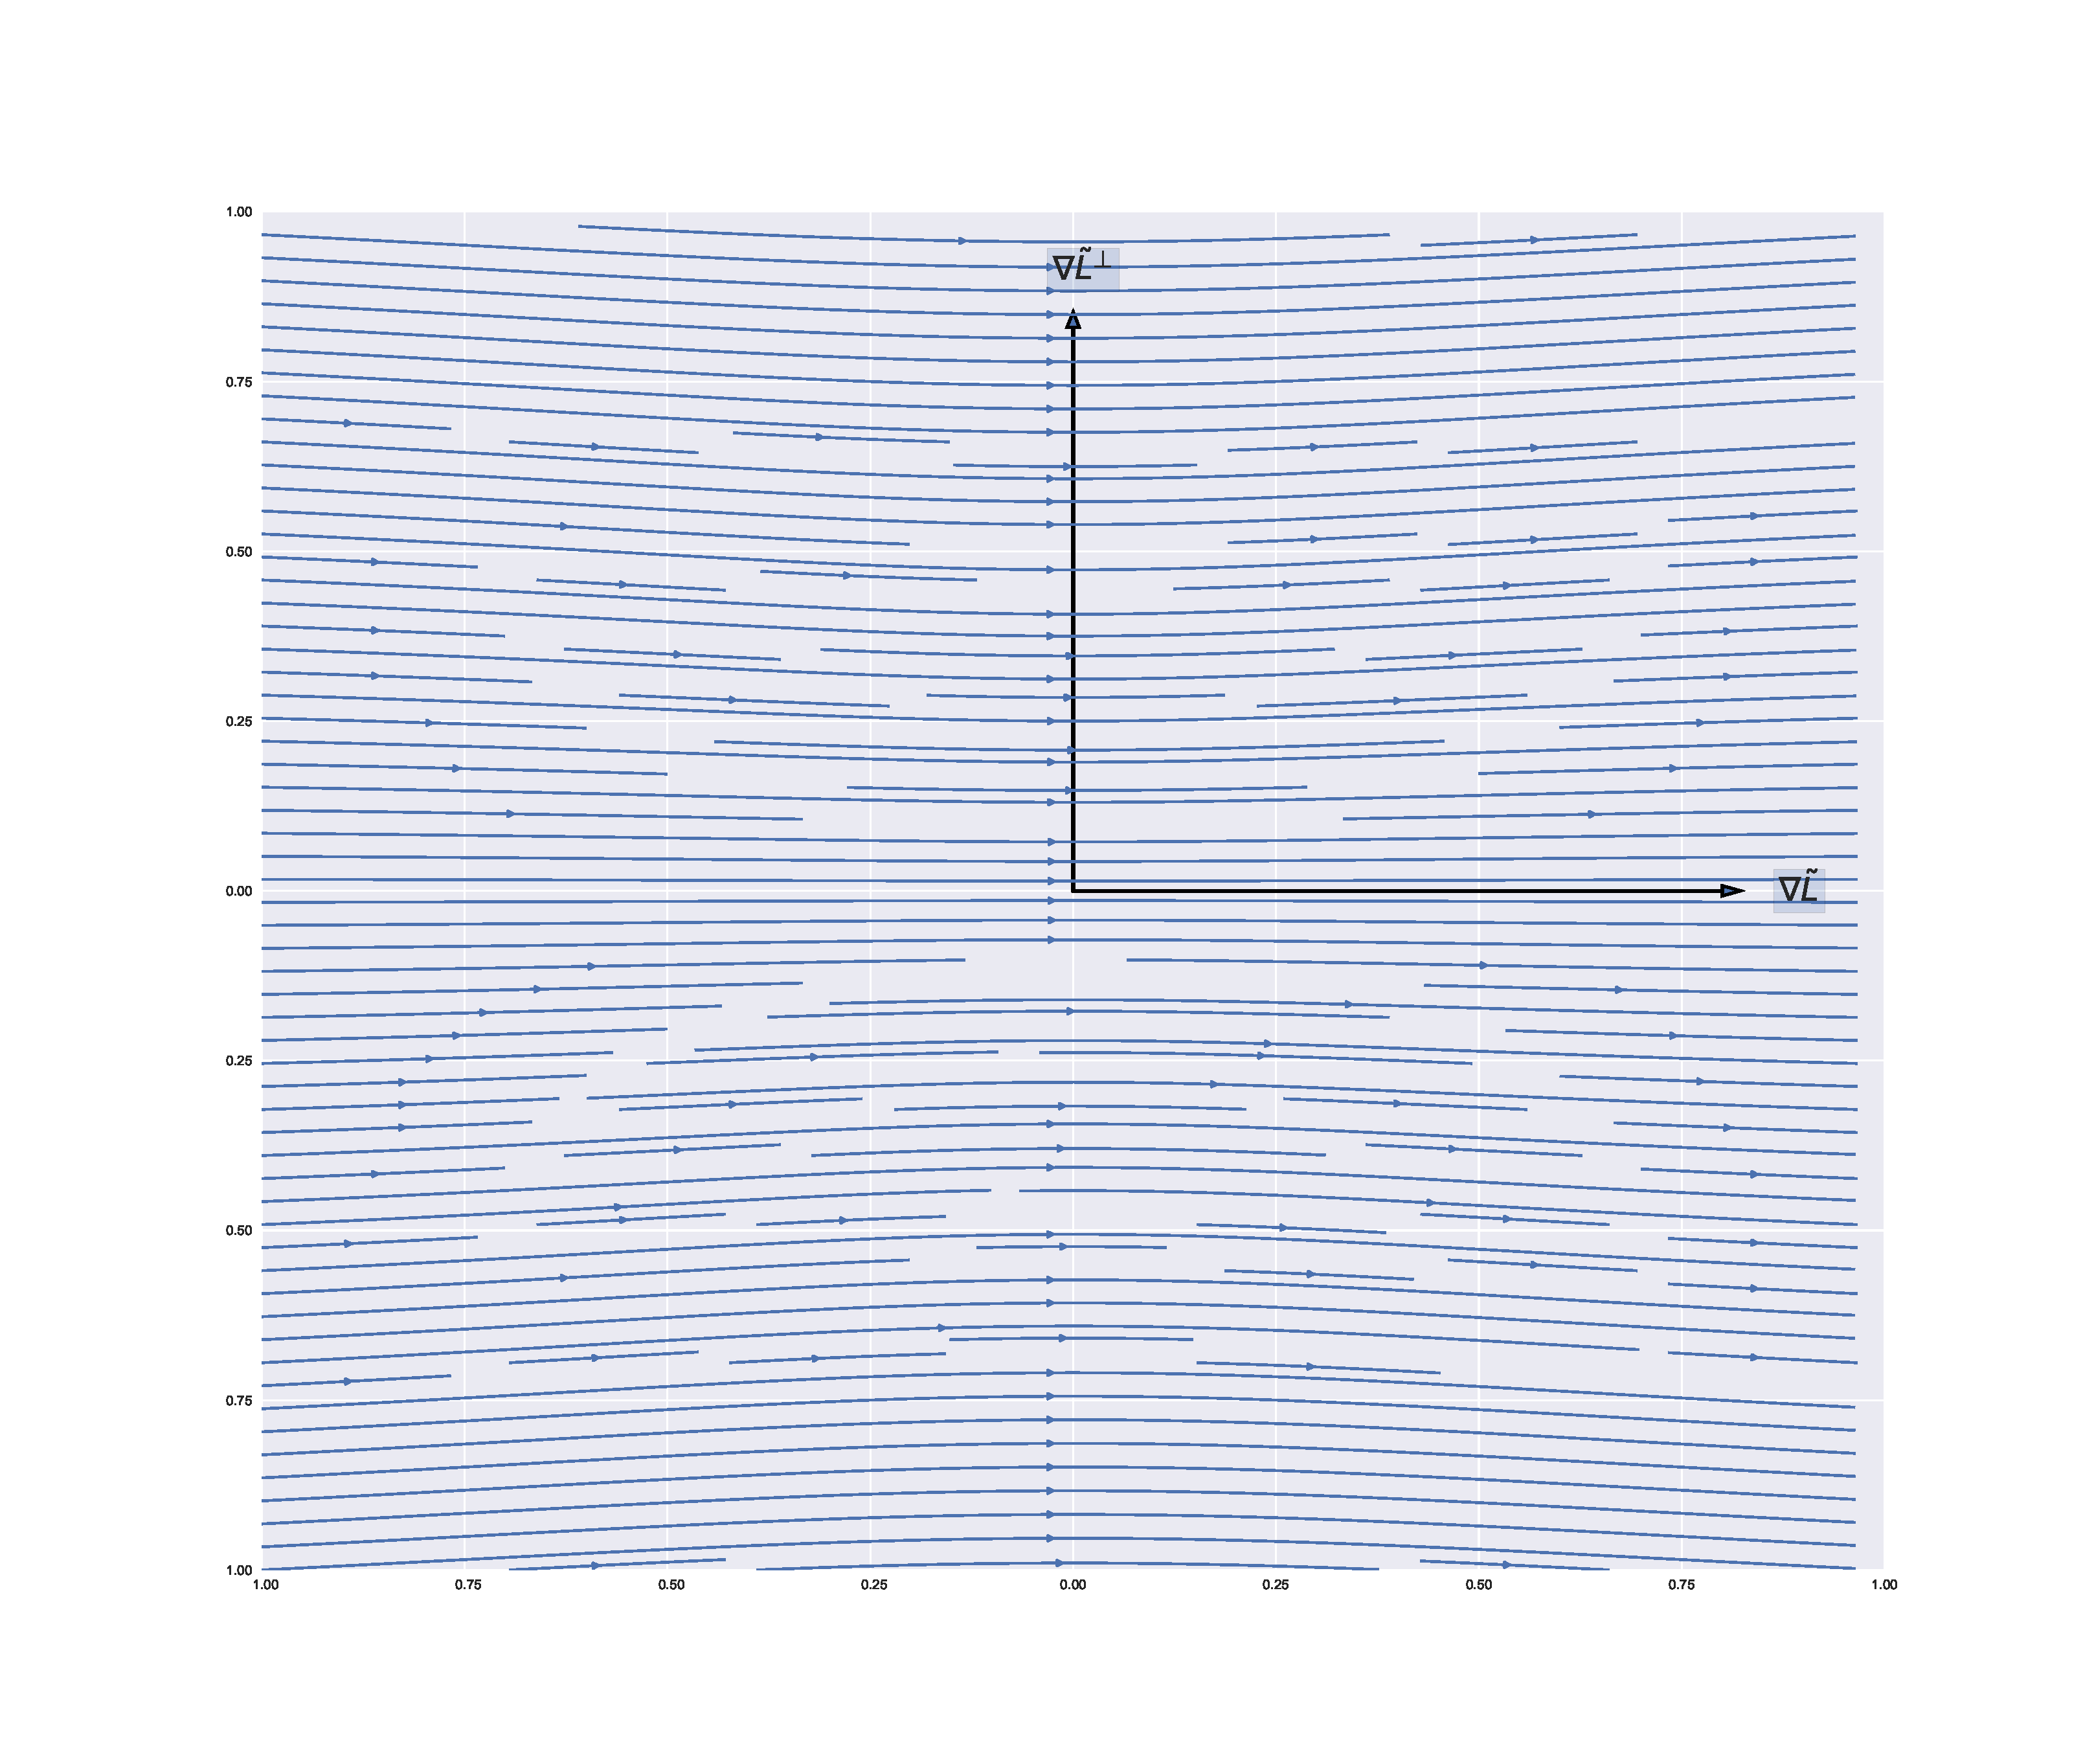
\includegraphics[width=\linewidth]{figures/dynamics_delta_1.pdf}
    % \endminipage\hfill
    \minipage{0.33\textwidth}
    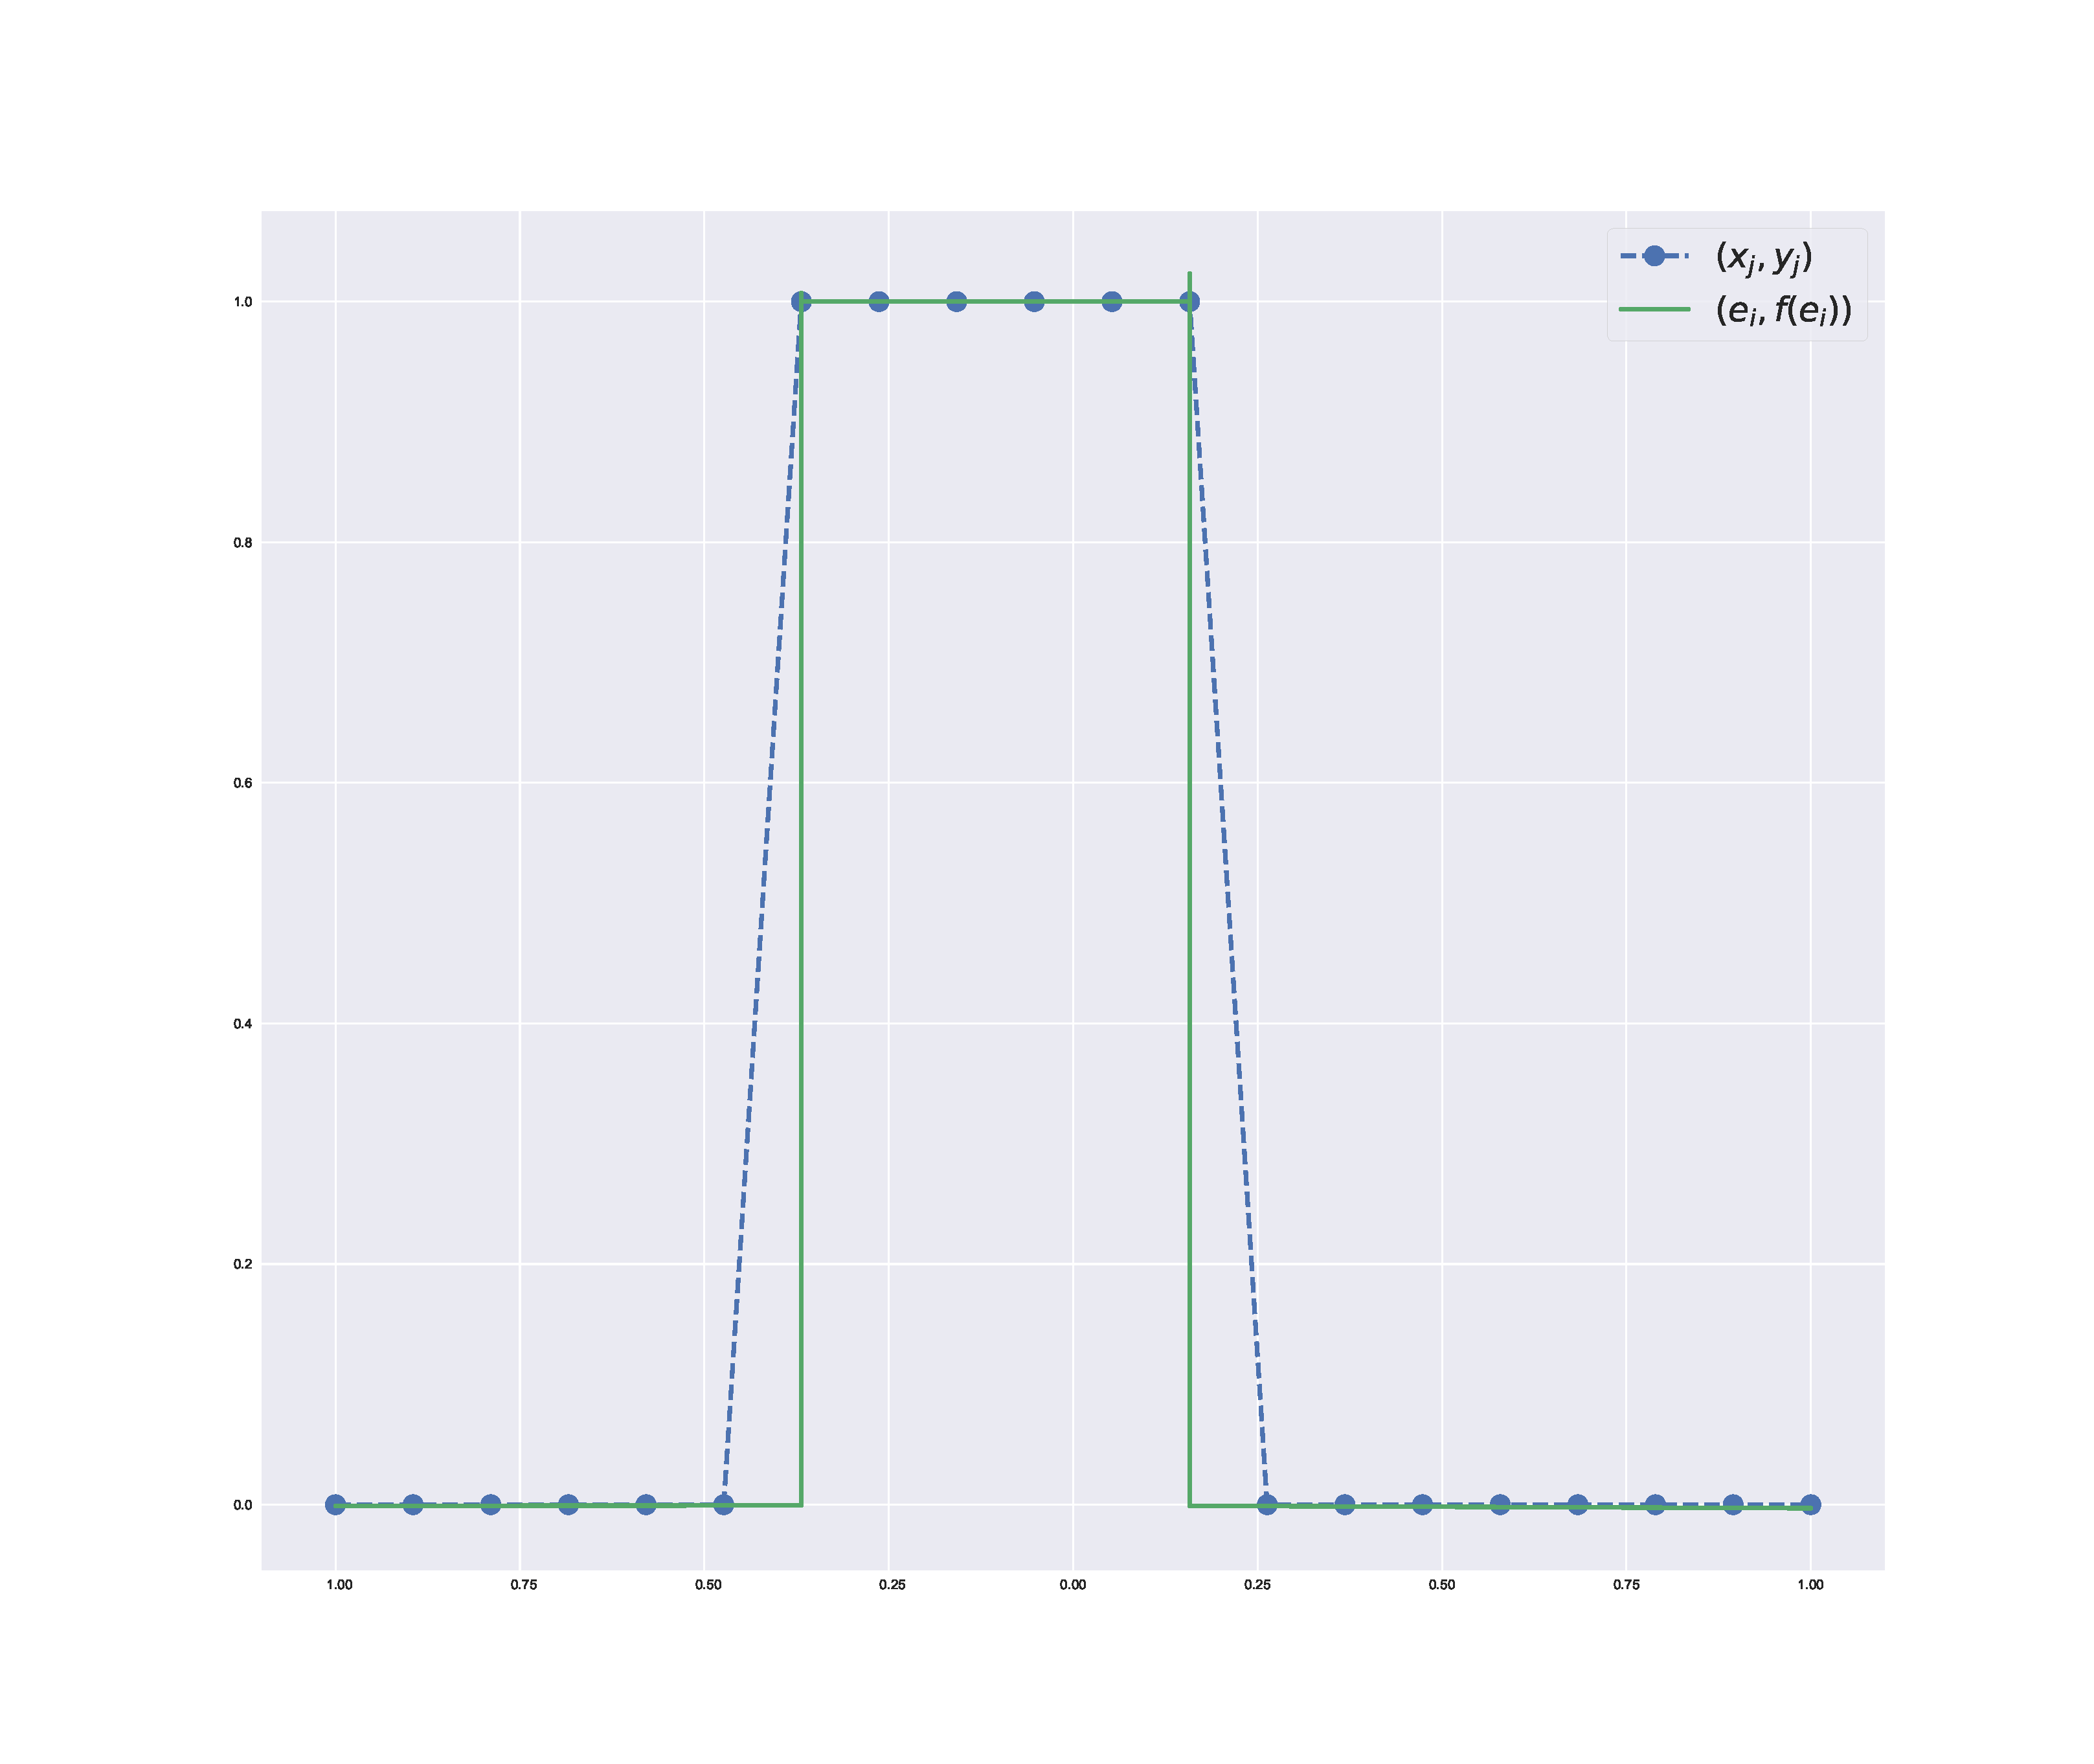
\includegraphics[width=\linewidth]{figures/same_init_different_func_square_1000.pdf}
    \endminipage
    
    \caption{The same initial function can yield very different results: the left image is the initial function for the two right ones. The initial parameters ($\bm a, \bm b, \bm c$) were the same as those in the middle image but scaled by a factor of 1000, 1000 and 0.001 respectively}
\end{figure}

\begin{figure}
    \centering
    \minipage{0.33\textwidth}
        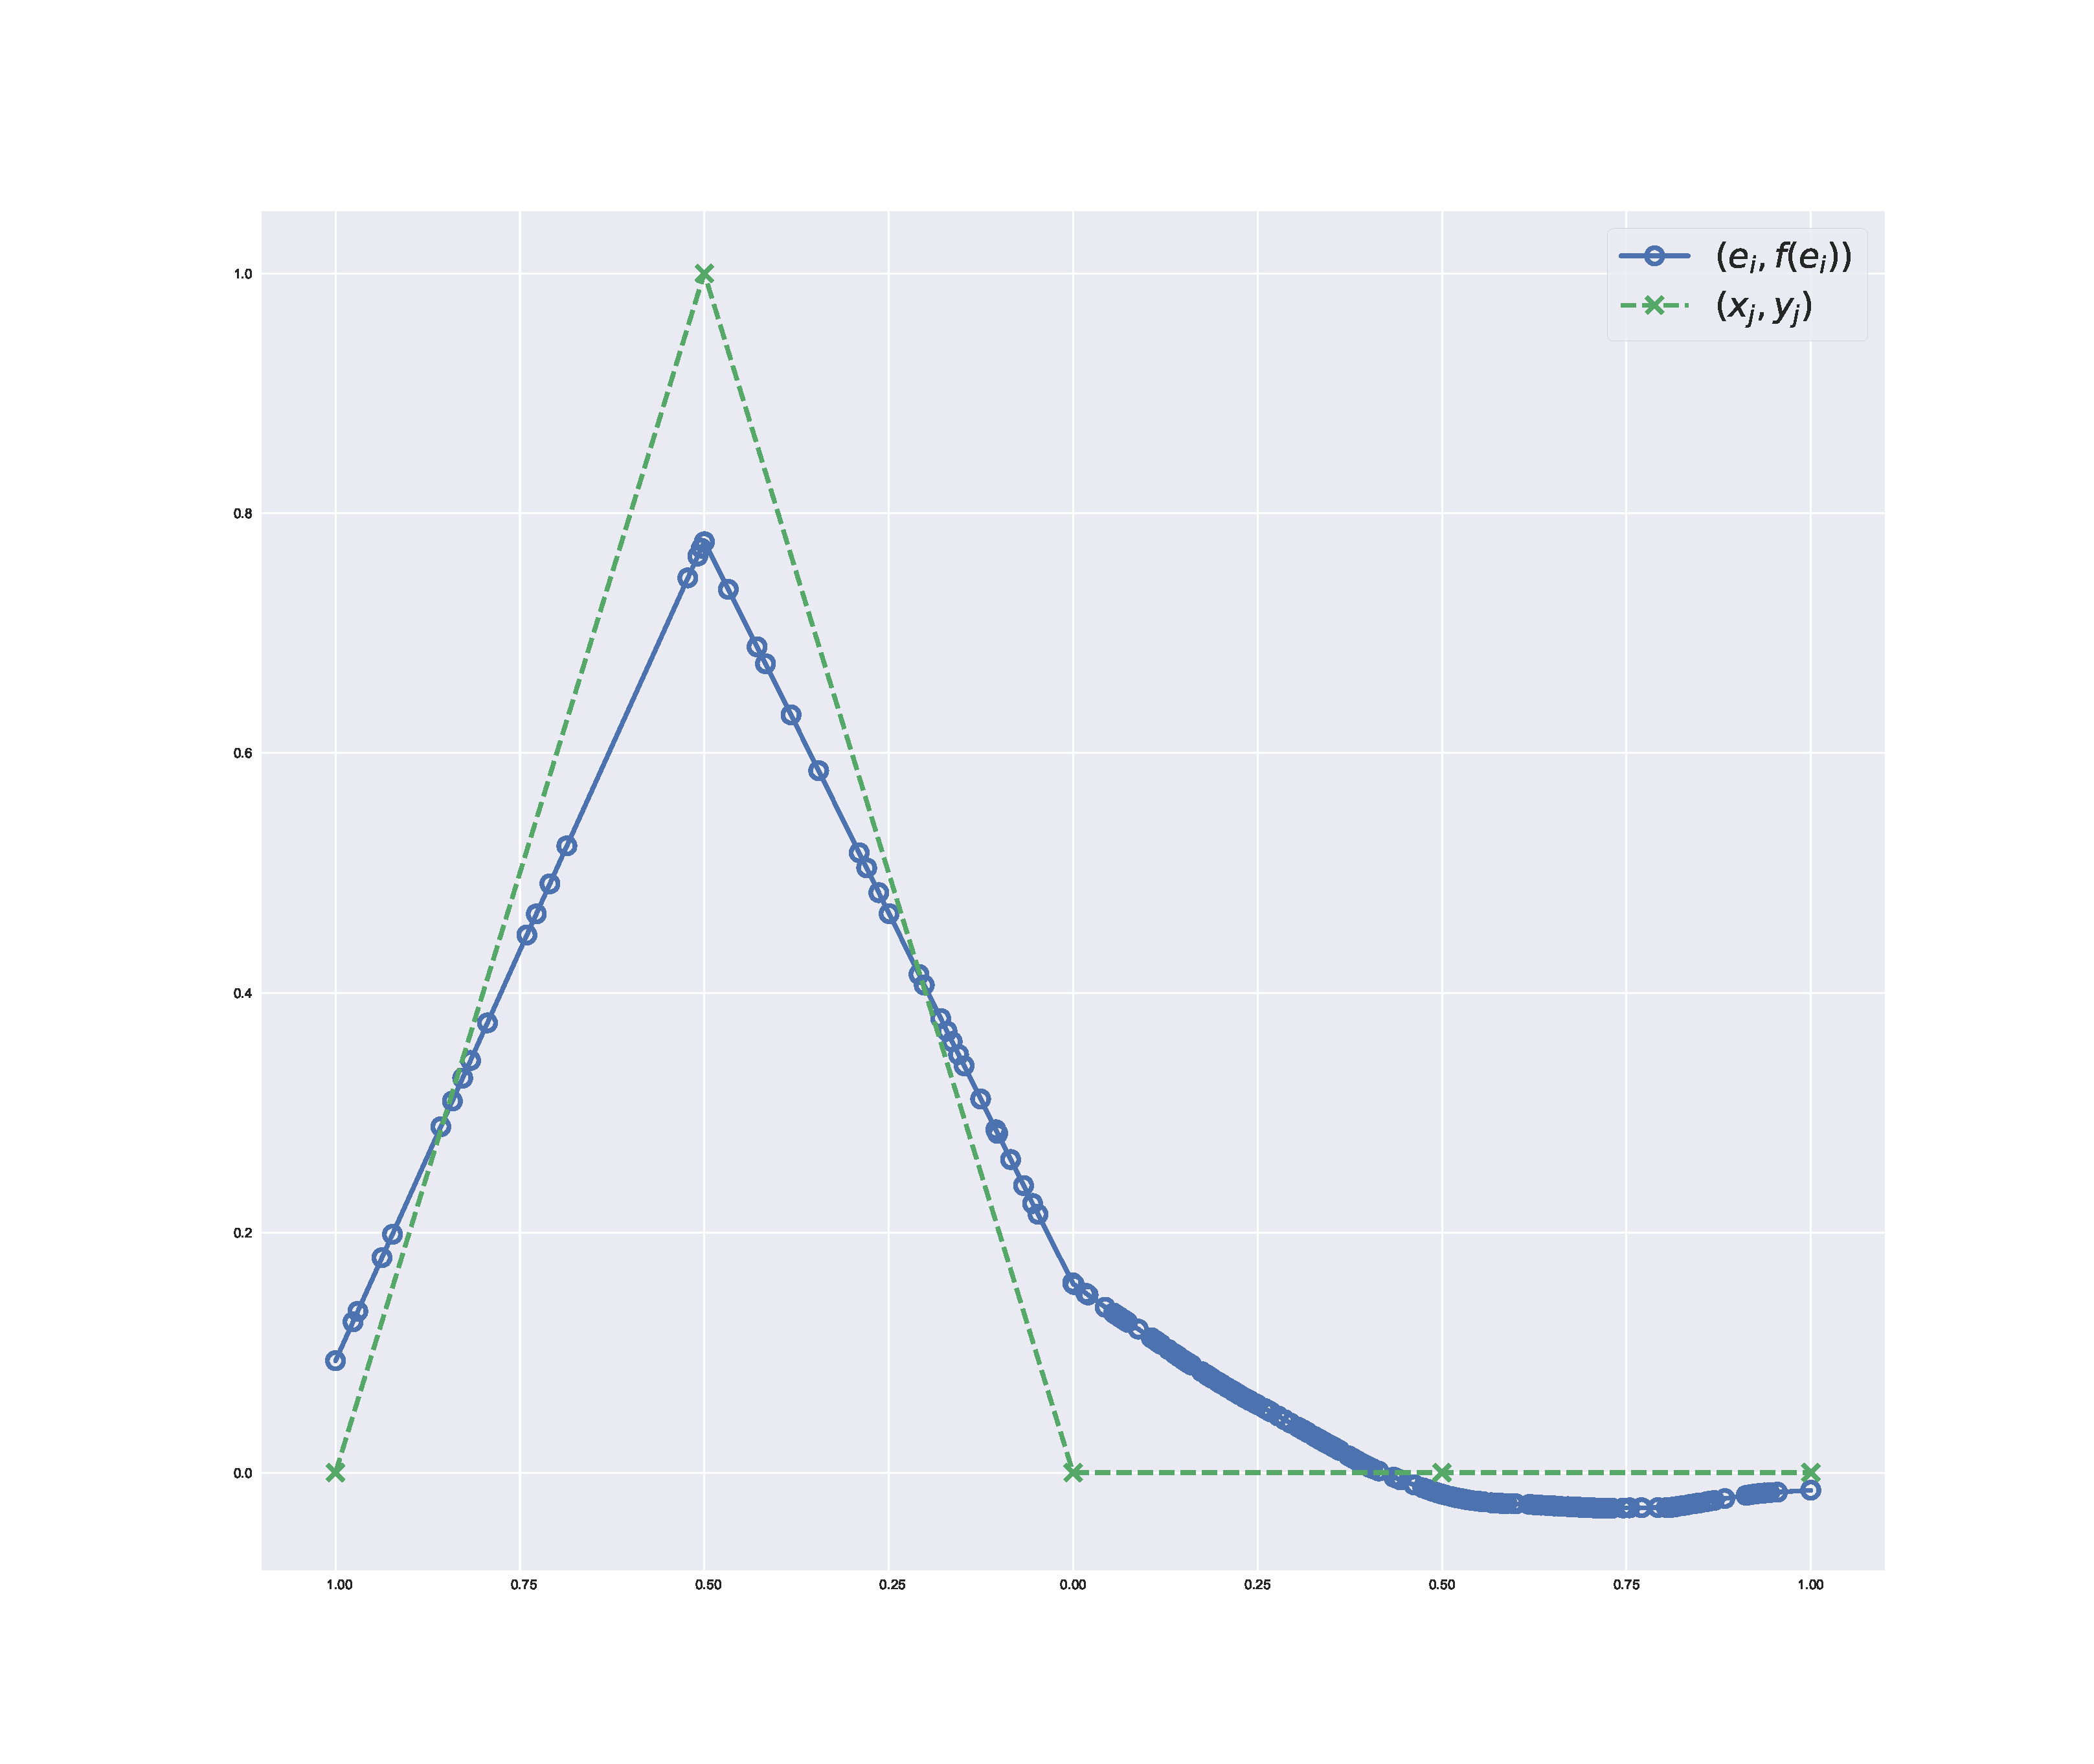
\includegraphics[width=\linewidth]{figures/reduced_gradient_recon.pdf}
    \endminipage
    \minipage{0.33\textwidth}
        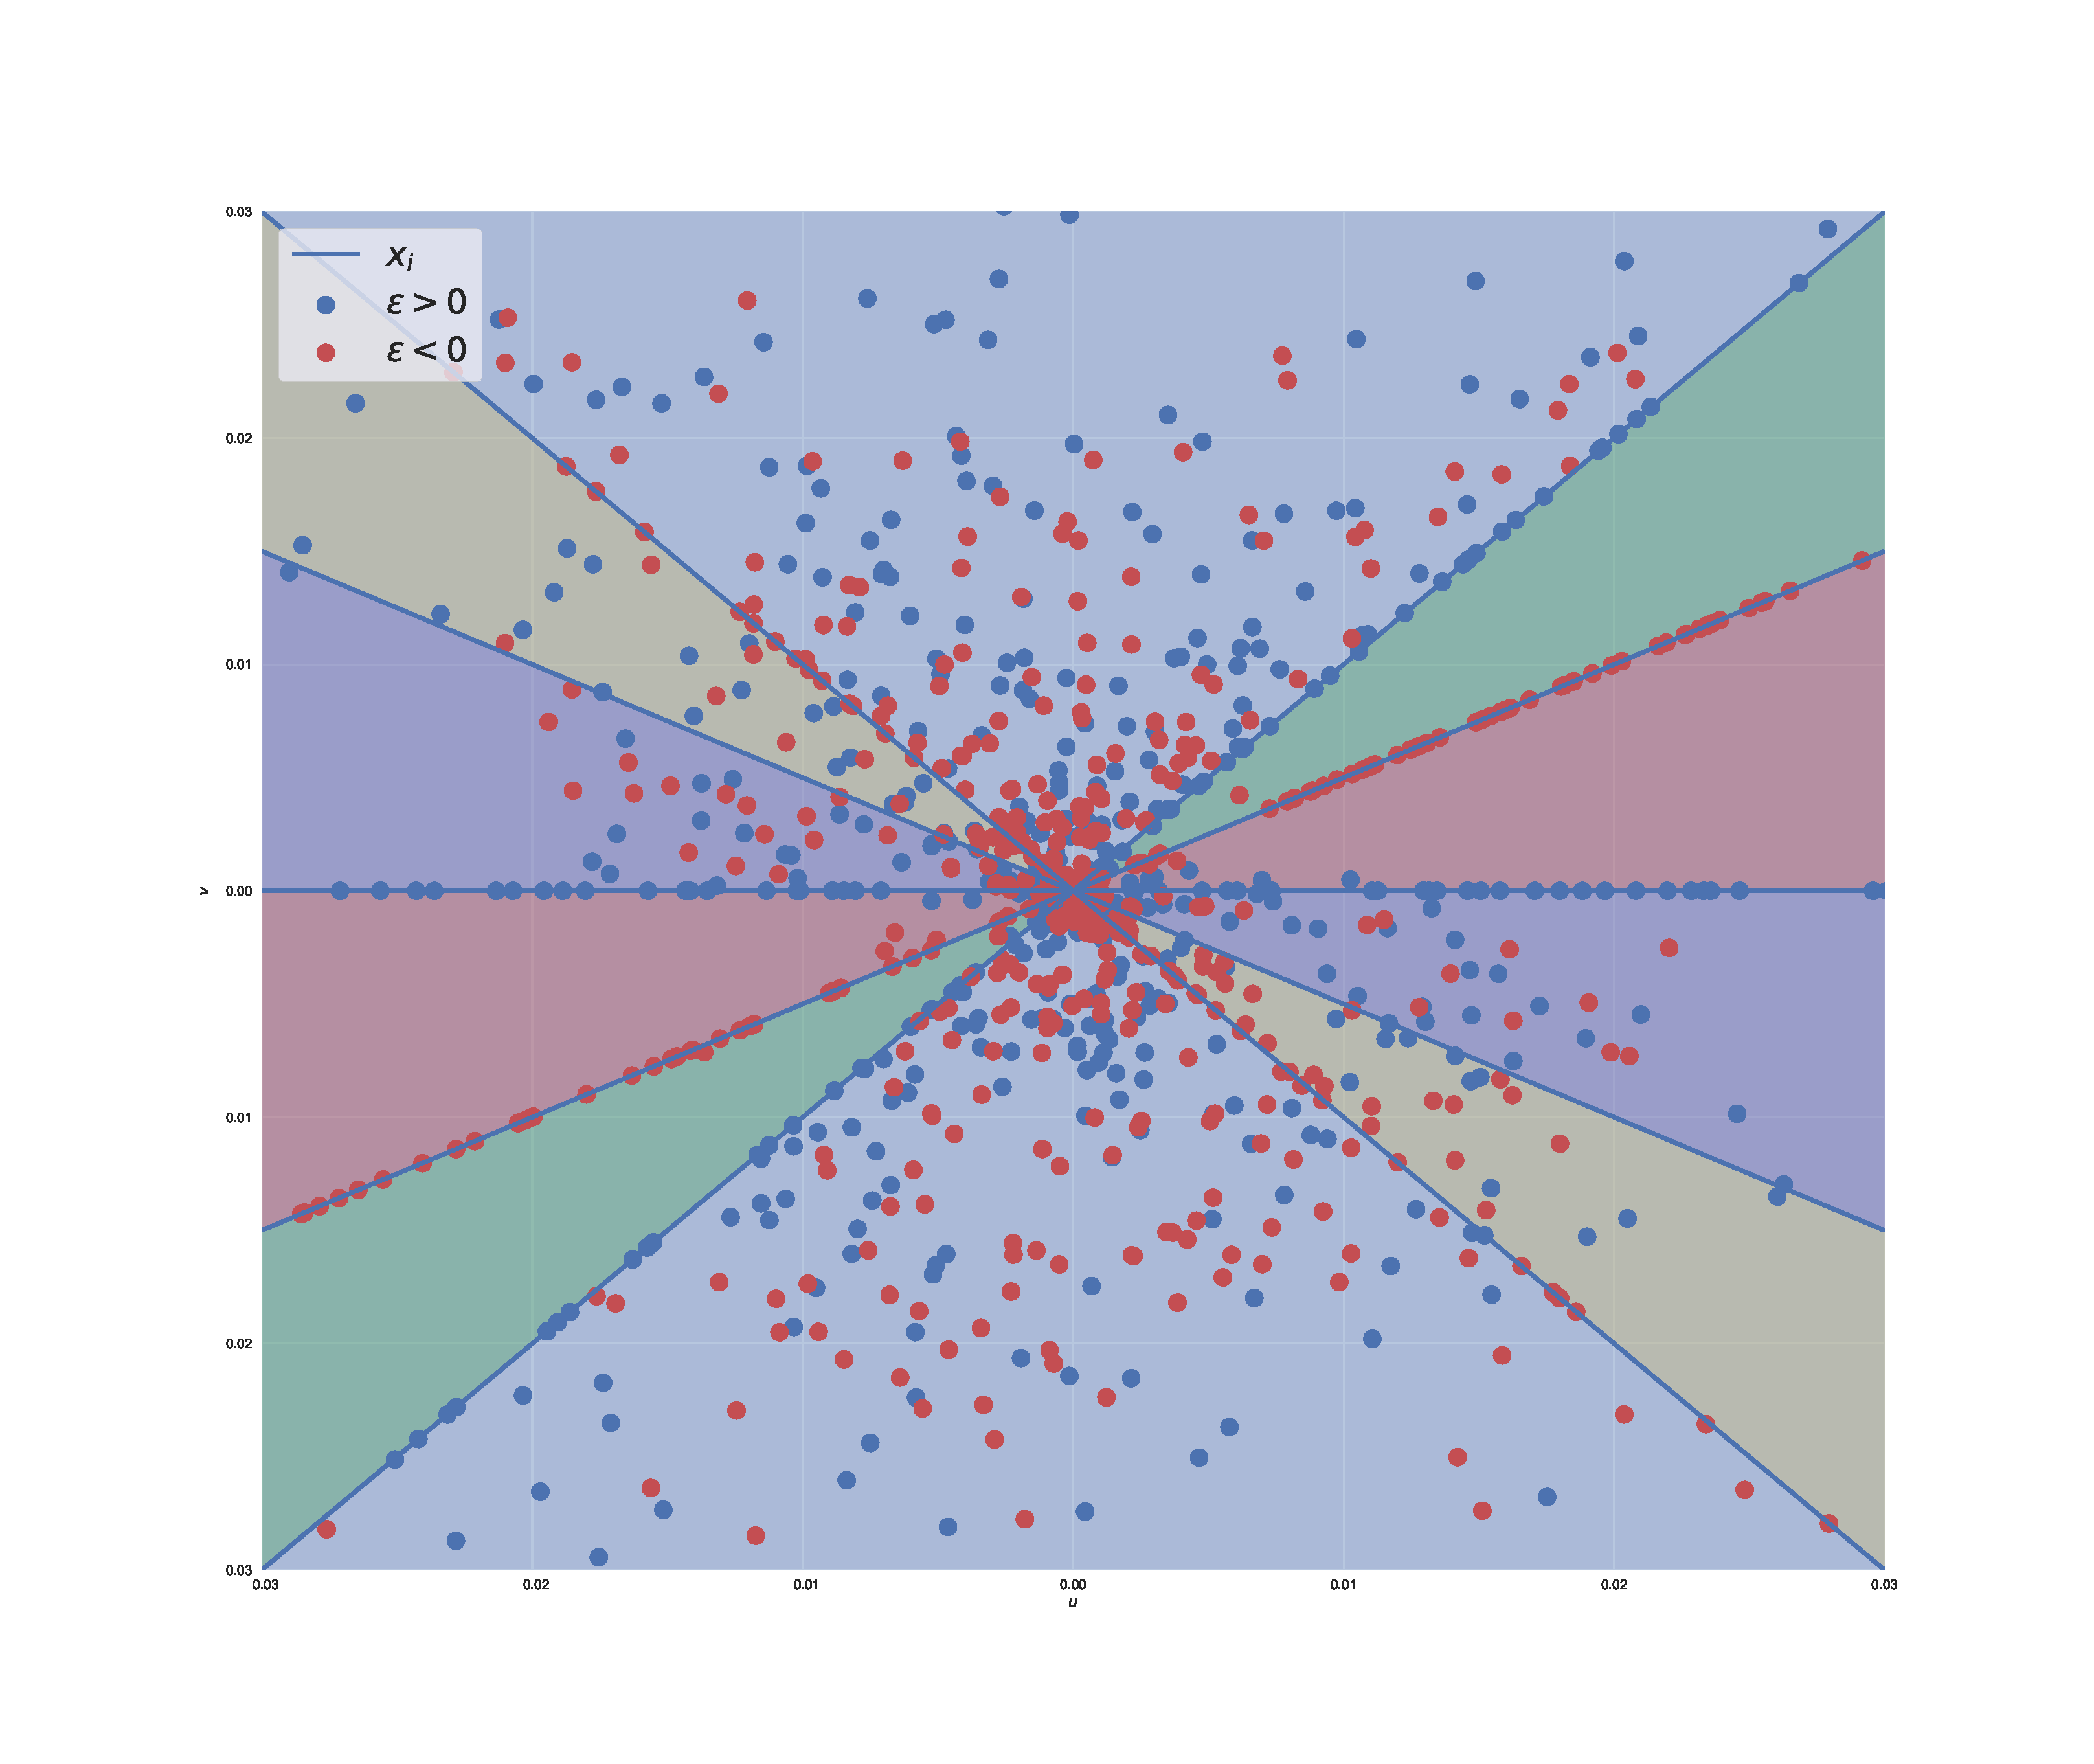
\includegraphics[width=\linewidth]{figures/reduced_gradient_phase.pdf}
    \endminipage
    \minipage{0.33\textwidth}
        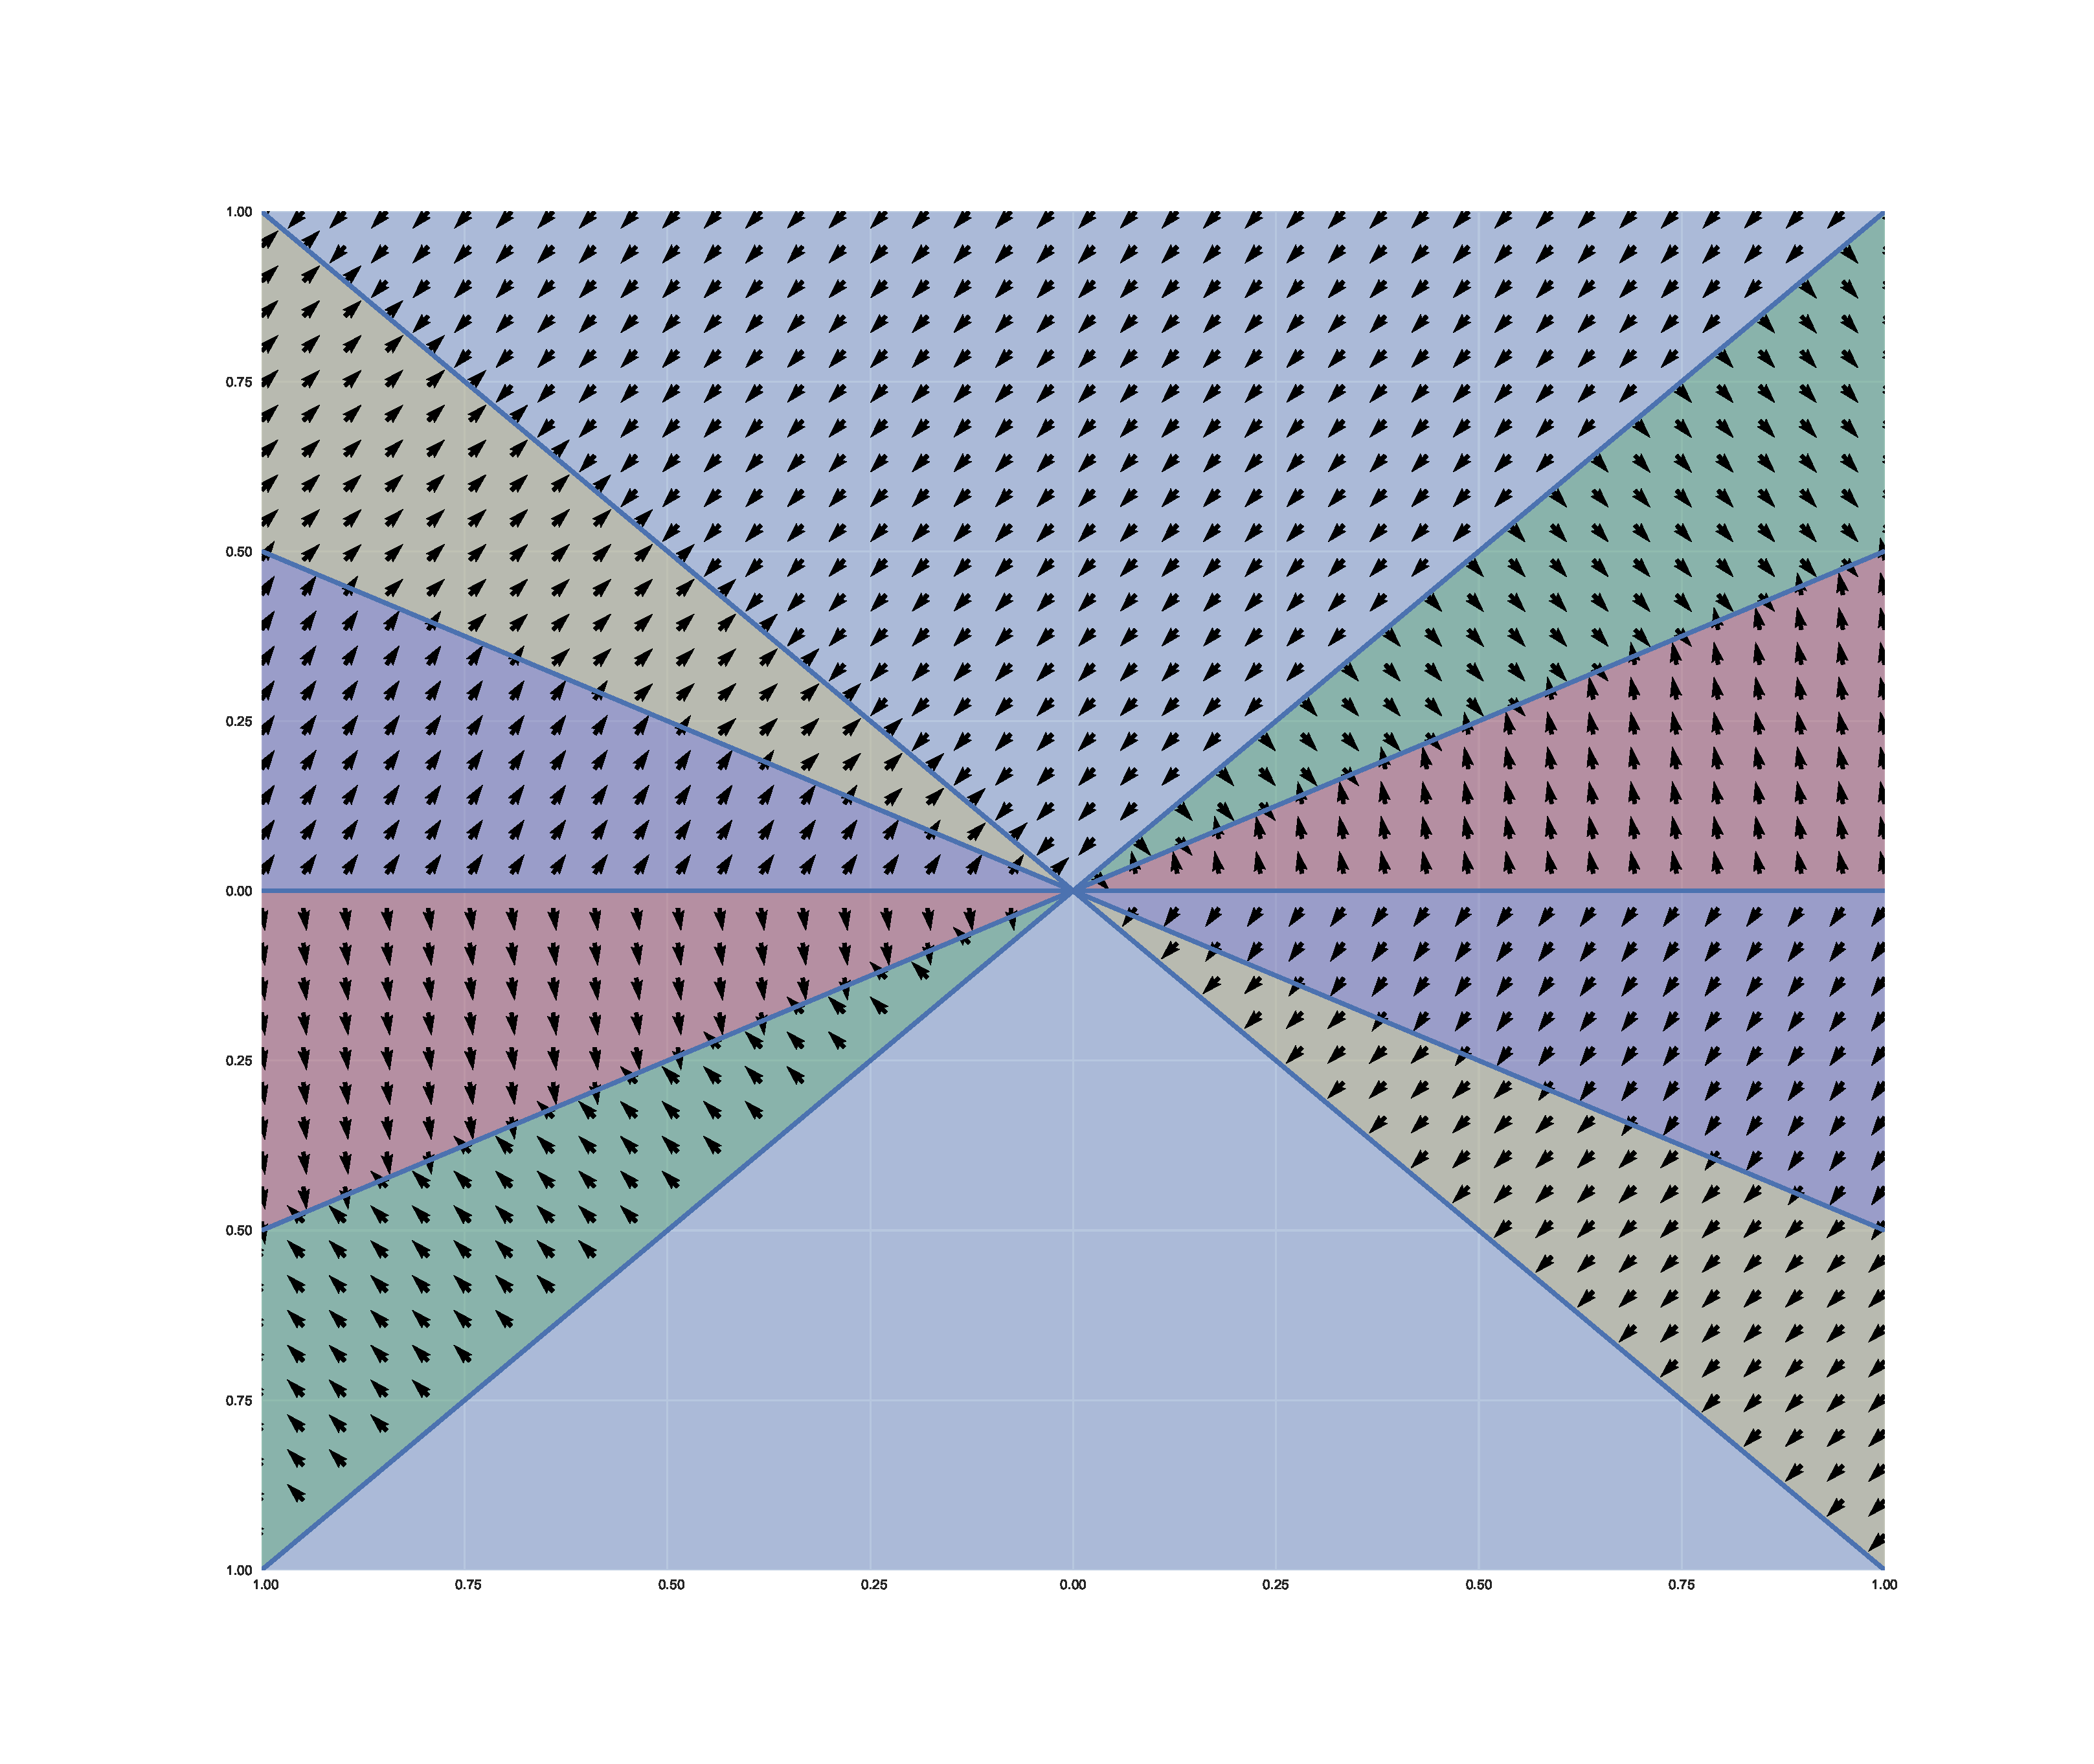
\includegraphics[width=\linewidth]{figures/reduced_gradient_vector_field.pdf}
    \endminipage\hfill
    \caption{The vector field of the gradient of the loss in reduced parameter space $\nabla \tilde{L}(\bm \xi)$. Note that the orientation of the arrow depends on the sign $\epsilon_i$ of a neuron. Thus, the gradient of the blue neurons are the arrows in the picture while the gradient of the red neurons point point in the opposite direction. We see in the middle image, that the neurons cluster on different samples depending on their sign.}
    \label{fig:reduced_grad}
\end{figure}